\section{\label{sec:vision}Visi\'on}

\subsection{Introducci\'on}
Como es sabido, el an\'alisis de im\'agenes es una tarea demandante en cuanto a complejidad
y tiempo de procesamiento requerido ya que involucra, entre otras cosas, operar sobre grandes matrices. Este motivo, nos llev\'o a 
implementar un m\'odulo de visi\'on separado del resto del software del robot.
En esta secci\'on exhibimos el sistema de an\'alisis de im\'agenes por 
el cual el robot en cuesti\'on da cuenta de la existencia o ausencia de 
elementos residuales en el entorno descripto.  El sistema se basa en la 
utilizaci\'on de una c\'amara de tipo webcam con una \'unica lente para 
obtener informaci\'on del ambiente. Esta informaci\'on es luego procesada 
por una computadora a bordo del robot utilizando un algoritmo de visi\'on 
cuyo \'unico objetivo es la detecci\'on de residuos 
en las im\'agenes obtenidas. Probamos este algoritmo dise\~nandolo para la detecci\'on de 
colillas de cigarrillo, vasos descartables y platos de pl\'astico. Para 
el desarrollo del algoritmo utilizamos la librer\'ia de visi\'on 
computacional OpenCV \cite{opencv_library} acompa\~nado de un sistema 
desarrollado en C++. Como plataforma utilizamos un sistema linux 
ubuntu corriendo en una netbook con procesador intel atom 
n450 y 1 gb de memoria RAM como se detalla en \ref{h_controlador_netbook}.
Esta secci\'on se divide en las siguientes partes: en la sub-secci\'on 2 mostramos  
los trabajos previos estudiados, en la sub-secci\'on 3 describimos el algoritmo de detecci\'on, 
en las secciones 4 y 5 explicamos los m\'odulos de predicci\'on y focalizaci\'on respectivamente mientras que en la 
sub-secci\'on 6 se muestran los resultados.En la sub-secci\'on 7 concluimos 
el cap\'itulo de visi\'on.

\subsection{Trabajos previos}
En esta secci\'on mostramos la informaci\'on obtenida a partir de 
trabajos anteriores relacionados con visi\'on computacional, 
procesamiento de im\'agenes y robots aut\'onomos.
 
	%~ \subsubsection{A tale of two object recognition methods for mobile 
	%~ robots- Arnau Ramisa}
	%~ Este trabajo trata el problema de reconocimiento de objetos en un 
	%~ contexto hogare\~no. El autor introduce este problema argumentando 
	%~ que existe una gran cantidad de algoritmos para reconocimiento de 
	%~ objetos pero pocos de estos son apropiados para robots moviles. 
	%~ Entre estos se destacan el m\'etodo de constelaci\'on utilizado con 
	%~ los detectores de puntos de interes de SIFT \cite{sift} y la bolsa 
	%~ de caracteristicas propuesto por Nister y Stewenius \cite[nister]. 
	%~ Con el objetivo de medir la performance de estos dos algoritmos, 
	%~ se recrea un ambiente hogare\~no compuesto por tres categor\'ias de 
	%~ objetos: texturados, no texturados, y con texturas repetitivas. 
	%~ Cada objeto utilizado tiene 20 im\'agenes de entrenamiento y cada 
	%~ categor\'ia contiene 3 objetos distintos. Luego se obtienen im\'agenes 
	%~ de prueba de estos objetos bajo condiciones de oclusi\'on, cambios 
	%~ de iluminaci\'on, distintas perspectivas y otros tipicos ruidos 
	%~ encontrados por un robot m\'ovil atravesando un entorno. De cada una 
	%~ de estas im\'agenes se consideraron dos versiones, una versi\'on con 
	%~ un recorte rect\'angular del objeto que incluye, inevitablemente, 
	%~ pixeles correspondientes al entorno de los objetos y una 
	%~ segmentaci\'on precisa utilizando los bordes de los objetos. Los 
	%~ resultados indican que utilizando el m\'etodo de Lowe se obtienen 
	%~ mejores resultados con las im\'agenes rect\'angulares ya que se todas 
	%~ las ocurrencias de los objetos texturados fueron reconocidas y  
	%~ tambi\'en algunos de los objetos con texturas repetitivas. Sin 
	%~ embargo, no se reconocieron objetos sin textura. Para el m\'etodo de 
	%~ la bolsa de caracteristicas 
	\subsubsection{\label{volunteer}Mobile Field Robot with Vision-Based Detection of Volunteer Potato Plants in a Corn Crop - FRITS K. VAN EVERT}
	El objetivo de este trabajo es la construcci\'on de un robot de 
	tama\~no reducido y de bajo costo capaz de detectar un tipo de 
	planta de papas (volunteer potato) en un campo de trigo y proporcionar control autom\'atico de esta planta. El inter\'es en 
	esta especie se debe a que esta planta resulta dif\'icil de controlar en las cosechas y favorece la 
	proliferaci\'on de otras sustancias que pueden perjudicar otros 
	cultivos. Con este prop\'osito, se utiliz\'o un cami\'on de juguete como 
	soporte para un robot aut\'onomo m\'ovil. Las partes de 
	radio-control del mismo fueron 
	removidas y remplazadas por micro-controladores para manejar la 
	direcci\'on y la velocidad del robot. Adem\'as se agregaron, como instrumentos de 
	sensado, una webcam est\'andar montada sobre un m\'astil a 
	una altura de 1.5m, un contador de revoluciones y un giroscopio de 
	estado s\'olido. Las im\'agenes tomadas por la webcam se procesaban 
	por una PC a bordo con un procesador Pentium M de 1.6 MHz. El control rob\'otico de \emph{volunteer potatoes} 
	involucr\'o al menos 3 grandes etapas: navegaci\'on a trav\'es del cultivo, detecci\'on 
	de plantas de papa y el control de las mismas.\\
	\indent En los campos de trigo la cosecha se dispone en filas 
	dejando espacio entre hilera e hilera para el paso del robot. Para 
	que este pueda navegar correctamente deb\'ia poder reconocer dichas 
	hileras de modo de orientarse correctamente en el cultivo. Ésto se 
	logr\'o mediante un algoritmo de visi\'on. Este comenzaba 
	tomando una imagen RGB de 320x240 de la c\'amara. Para separar las 
	plantas del fondo se tom\'o el doble del valor del canal verde (G)  y se 
	sustraen los canales rojos y azules (R y B respectivamente) (2G -R - B). Pixeles con un 
	valor mayor a cierto umbral son considerados planta y todos los 
	dem\'as, fondo. En un segundo paso de procesamiento, se detectaron las 
	filas de plantas utilizando un algoritmo inspirado en la 
	transformada de Hough \cite{hough62}. Este dibujaba l\'ineas imaginarias sobre la 
	imagen segmentada y establec\'ia un puntaje para cada una seg\'un 
	cuantos pixeles blancos (plantas) cubr\'ian. Estos puntajes se 
	convert\'ian en valores de pixeles de una nueva imagen en donde la 
	coordenada vertical de cada pixel correspond\'ia con la pendiente de 
	la l\'inea imaginaria y donde la coordenada horizontal con la 
	intersecci\'on con el eje de coordenadas. Las hileras de plantas 
	contribu\'ian pixeles a varias l\'ineas imaginarias y aparec\'ian en la 
	nueva imagen como \'areas con pixeles brillantes. Se utilizaron las 
	operaciones de threshold y dilataci\'on para combinar estas \'areas 
	brillantes en un \'unica regi\'on contigua de la cual se 
	extra\'ia el centro de gravedad para representar una hilera de 
	plantas. Ya que el ruido pod\'ia ocasionar el reconocimiento de 
	hileras de plantas inexistentes se utilizaron algunas reglas 
	sencillas para validar estas detecciones. Dos ejemplos de estas 
	reglas son ``las hileras de plantas deben estar a uno de los dos 
	costados del robot'' y ``las hileras deben ser paralelas entre s\'i''.
	Luego, la orientaci\'on del robot se establec\'ia seg\'un la pendiente de 
	estas l\'ineas.\\
	\indent Para la detecci\'on de las plantas \emph{volunteer potato} se 
	utiliz\'o una segunda c\'amara ubicada a una menor altura para obtener 
	mayor resoluci\'on sobre las plantas en s\'i. El algoritmo consist\'ia en 
	extraer las siguientes caracter\'isticas de las im\'agenes: 
	\begin{enumerate}
	\item{promedio de rojo para pixeles de planta.}
	\item{promedio de verde para 
	pixeles de planta.}
	\item{promedio de azul para pixeles de planta.}
	\item{n\'umero total de pixeles de planta en la imagen binaria.}
	\item{n\'umero total de pixeles de contorno en la imagen binaria.}
	\item{n\'umero total de pixeles de borde en la imagen Canny binaria.}
	\end{enumerate} Estas 
	caracter\'isticas se relacionan al color (1,2 y 3), tama\~no (4), figura 
	(combinaci\'on de 4 y 5) y textura (6).  Utilizando la misma f\'ormula 
	(2G -B -R) y la operaci\'on de threshold se segment\'o nuevamente la imagen 
	 en pixeles de planta o fondo. Sobre esta imagen se calcul\'o el 
	 promedio de rojo, azul y verde para las caracter\'isticas 1,2 y 3. 
	 Contando el n\'umero de pixeles planta ( pixeles considerados como 
	 correspondientes a los de una planta) en la misma 
	 imagen se obtuvo la caracter\'istica 4. Para la caracter\'istica 5 
	 se extraen los contornos de esta imagen y se cuenta el n\'umero de 
	 pixeles plantas contenidos en ellos. Finalmente, para la caracter\'istica 6 se 
	 repite este \'ultimo procedimiento extrayendo los bordes de la 
	 imagen pero,  
	 utilizando una implementaci\'on del algoritmo de Canny 
	 \cite{Canny:1986:ACA}. Se esperaba que el n\'umero de pixeles de 
	 borde sea mayor si se trata de una planta de papa ya que esta 
	 contiene un n\'umero mayor de hojas peque\~nas que se solapan entre s\'i 
	 mientras que las de trigo s\'olo contienen algunas pocas hojas. 
	 Paraf 
	 clasificar las im\'agenes se us\'o un set de im\'agenes de entrenamiento
	 que fueron clasificadas manualmente seg\'un si conten\'ian 
	 plantas de papa o no. Luego se entren\'o un 
	 clasificador de discriminante lineal de Fisher \cite{HastieEtAl2008} para distinguir 
	 entre im\'agenes que contienen plantas de papa de las que no.\\
	 \indent Para poner a prueba el algoritmo se tomaron dos sets de 
	 im\'agenes capturando el recorrido del mismo robot aut\'onomo a 
	 trav\'es de un campo de trigo. La tasa global de error para el 
	 clasificador fue de 1.5\% en el primer set y 10.6\% en el 
	 segundo. En cuanto al rendimiento en la navegaci\'on, el robot 
	 fue capaz de recorrer con \'exito 120m de hileras de cultivo con 
	 una velocidad promedio de $0.67$ m/s. El autor remarc\'o el alto 
	 tiempo de procesamiento requerido por el detector de plantas de 
	 papa ya que este baj\'o la tasa de cuadros del algoritmo de 
	 navegaci\'on de 30 a 8 cuadros/segundo. Por dicho motivo se 
	 redujo la velocidad de desplazamiento del robot a 0.2 m/s para 
	 que fuera capaz de capturar correctamente todas las plantas. 
	 El mecanismo de control no fue implementado pero se incluy\'o un 
	 speaker que reprodujo un sonido cuando \'este encontraba una planta 
	 del tipo buscado. Los algoritmos de visi\'on utilizados fueron 
	 desarrollados usando Matlab con la librer\'ia Delft \cite{DipLib}.
	 
	\subsubsection{Review of shape representation and description techinques - Dengsheng Zhang}
El objetivo de este trabajo es realizar un resumen de las t\'ecnicas m\'as 
importantes en cuanto a la representaci\'on y descripci\'on de figuras o 
formas.
Al clasificar dichas t\'ecnicas el autor sugiere una primera 
sub-divisi\'on en 2 grupos: m\'etodos basados en contornos y m\'etodos basados en regiones. 
Los primeros se caracterizan por extraer  la informaci\'on 
solo del contorno mientras que los segundos, de la regi\'on completa abarcada
por la figura. Dentro de cada clase se dividen en t\'ecnicas 
estructurales o t\'ecnicas globales de acuerdo a si la figura se 
representa como un todo o por segmentos y secciones respectivamente. 
Exhibimos la jerarqu\'ia completa en la figura \ref{fig:review_shape}.\\
\indent Dentro de la categor\'ia de los basados en contornos, en la sub-categor\'ia de globales, los m\'etodos suelen computar vectores de 
propiedades num\'ericas extra\'idas de la informaci\'on del borde de una 
figura. La comparaci\'on entre formas se realiza 
generalmente utilizando m\'etricas de distancia, como la distancia euclideana. Ejemplos de m\'etodos sencillos que caen dentro de esta 
categor\'ia son \textit{area, circularidad( $perimetro^2 / area$), 
excentricidad ( longitud del eje mayor / longitud del eje menor)}. Otros m\'etodos 
de la misma familia pero m\'as complejos son los m\'etodos basados en la correspondencia de puntos. En estos m\'etodos se trata a cada punto como una caracter\'istica de la figura que compone. La distancia de \textit{ Hausdorff} es una t\'ecnica cl\'asica de esta categor\'ia. Dadas dos formas representadas
por dos sets de puntos $A={x_1,x_2...x_n}$ y $B={y_1,y_2...y_n}$ la distancia Haussdorf se define como 
\[
	 d_{\mathrm H}(A,B) = \max\{\,\sup_{x \in A} \inf_{y \in B} d(x,y),\, \sup_{y \in B} \inf_{x \in A} d(x,y)\,\}\mbox{,}
\] 

La comparaci\'on de figuras usando distancia Hausdorff resulta sensible 
al ruido y a peque\~nas alteraciones en dos formas iguales. Existen otros m\'etodos basados
en \textit{firma de contorno} que  representan una figura con una 
funci\'on uni-dimensional derivada de la informaci\'on del borde de la 
misma, 
algunos son \textit{perfil centroidal, coordenadas complejas y distancia al centroide}. Estos m\'etodos deben ser normalizados para compensar
traslaciones o escalas lo que los hace relativamente costosos. Ésto, sumado a la sensibilidad al ruido y a peque\~nos cambios en los bordes, hace que el m\'etodo 
no sea lo suficientemente robusto y que necesite de procesamiento adicional. Otra familia de descriptores se basa en los 
\textit{Momentos de borde}. Dada una parametrizaci\'on como una funci\'on 
uni-dimensional $z (i)$, se define el momento \textit{r}-\'esimo \textit{$m_r$} 
y el momento central $\mu_r$ como:
\[
	m_r=\frac{1}{N} \sum_{i=1}^{N}{[z(i)]^r}\ \ \ \ \
	\mu_r=\frac{1}{N} \sum_{i=1}^{N}{[z(i) - m_1]^r}
\]

donde N es el n\'umero de puntos de borde. El momento normalizado $\bar{m_r}=m_r / (\mu_2)^{r/2}$
es invariante frente a traslaciones, rotaciones y escalamientos. Sin 
embargo, los momentos de alto orden
son dif\'iciles de asociar con interpretaciones f\'isicas del contorno.\\
\indent La otra sub-categor\'ia dentro de los m\'etodos basados en contornos es la de los m\'etodos estructurales.
En estos m\'etodos se suele descomponer un contorno en segmentos de bordes llamado primitivas. Los m\'etodos estructurales
entonces se diferencian entre s\'i de acuerdo a la definici\'on y organizaci\'on de estas primitivas. Algunos m\'etodos
de descomposici\'on son: aproximaci\'on por pol\'igonos, descomposici\'on por curvatura, y ajuste de curva. El resultado
de la descomposici\'on se codifica como una cadena $S=\{s_1,s_2...s_n\}$ donde $s_i$ puede ser un lado de un pol\'igono, una 
arista cuadr\'atica, una funci\'on spline, etc. Adem\'as, $s_i$ puede 
contener varios atributos como longitud, orientaci\'on o curvatura 
promedio, entre otros.
Un m\'etodo en esta l\'inea es por ejemplo el de c\'odigo en cadena, en el 
cual se describe un objeto por una serie de segmentos de longitud 
unitaria y una orientaci\'on determinada. 
En su implementaci\'on se superpone una imagen con una grilla y se aproximan los puntos del contorno al 
punto de la grilla m\'as cercano. Luego se selecciona un punto de 
partida y se codifica una secuencia, estableciendo la direcci\'on del segmento
que conecta un punto con el siguiente seg\'un la direcci\'on de \'este en 
la grilla (respecto del punto  anterior). Para la comparaci\'on de dos
contornos es necesario realizar normalizaciones ya que el punto de 
partida puede variar y frente a un cambio de escala pueden parecer 
contornos distintos. Otros m\'etodos en esta sub-categor\'ia pueden ser el de la descomposici\'on polin\'omica o la descomposici\'on en curvas suaves. \\
\indent Dentro de la categor\'ia de los m\'etodos basados en la regi\'on 
de una figura y la sub-categor\'ia de globales podemos encontrar los \textit{momentos Hu}.
Un momento de Hu de un contorno 2D se define como:
\[
	m_{pq}=\sum_{x}{\sum_{y}{x^py^qf(x,y)}}
\]

Usando combinaciones lineales de momentos de Hu de \'ordenes bajos 
(valores de p y q menores a 2) se obtiene un descriptor 
invariante frente a rotaciones, traslaciones o escalamientos. Sin 
embargo esta t\'ecnica prob\'o servir s\'olo 
para figuras simples ya que en formas m\'as complejas no tiene un buena 
rendimiento. Otros m\'etodos en esta
sub-categor\'ia pueden ser \textit{momentos algebraicos} o \textit{descriptor general de Fourier}. En la otra sub-categor\'ia de m\'etodos
estructurales se destaca la \textit{envoltura convexa}. La 
\textit{envoltura convexa} de un set de puntos es la m\'inima regi\'on que contiene 
dichos puntos y es convexa. Este m\'etodo obtiene dicha regi\'on y la compara con el contorno original obteniendo una serie de peque\~nas
componentes que marcan las deficiencias de concavidad del contorno. La 
figura en cuesti\'on puede entonces representarse utilizando estas componentes.
Finalmente la comparaci\'on entre dos contornos representados con esta 
t\'ecnica resulta en la comparaci\'on de grafos(caracterizando las 
deficiencias mencionadas) lo cual es otro
problema a resolver por s\'i mismo. Adem\'as, m\'etodos en esta familia son dif\'iciles y complejos de implementar.\\
\indent Como conclusi\'on, el autor establece que los m\'etodos basados en contorno son m\'as populares ya que est\'an m\'as relacionados
a la percepci\'on humana y que para muchas aplicaciones es s\'olo necesario la informaci\'on sobre el contorno y no sobre el interior del mismo.
Sin embargo, tambi\'en establece que como solo usan parte de una figura, son m\'as sensibles al ruido y peque\~nas variaciones.

\begin{figure}[tpb]
\begin{center}
  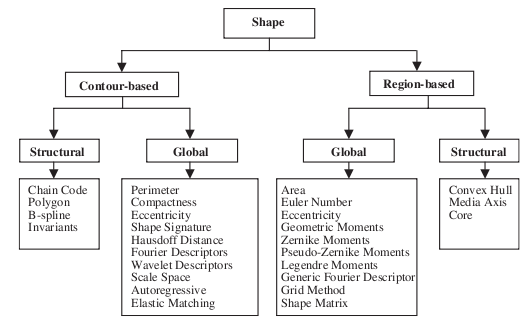
\includegraphics[scale=0.55]{vision/figures/shapess.png}
\end{center}
  \caption[t\'ecnicas de descripci\'on de figuras]
  {Clasificaci\'on de las t\'ecnicas de descripci\'on y representaci\'on de figuras}
  \label{fig:review_shape}
\end{figure}

% sidewalk following
	\subsubsection{\label{sec:sidewalk} Sidewalk Following Using Color Histograms - John S. Seng}
	Este trabajo describe un algoritmo  para detectar y seguir 
	veredas o \'areas transitables en un video filmado, con el objetivo de 
	lograr la navegaci\'on aut\'onoma de un robot dentro del 
	campus de una universidad. La plataforma en la cual se tomaron los 
	videos estaba 
	compuesta de una silla de ruedas motorizada controlada por una CPU 
	a bordo corriendo un sistema operativo Linux. El robot ten\'ia una 
	\'unica c\'amara NTSC que prove\'ia im\'agenes color con una tasa de 15 
	cuadros por segundo. Todos los videos de prueba fueron tomados 
	utilizando esta plataforma conduci\'endola remotamente por un 
	operador a trav\'es de un sistema de radio.\\
	\indent El algoritmo en cuesti\'on utilizaba histogramas 2D de los 
	canales de tono y saturaci\'on de los pixeles para modelar las \'areas
	transitables y las no transitables. Se utilizaba un \'area de 
	entrenamiento ubicada directamente en frente del robot en la cual se 
	asum\'ia que 
	no hab\'ian obst\'aculos y conten\'ia pixeles representativos del \'area que 
	estaba transitando. Esta \'area de entrenamiento se utilizaba para 
	actualizar uno de los 4 histogramas que modelaban el \'area 
	transitable. Adem\'as, se manten\'ia un histograma que modelaba el
	\'area no transitable o fondo de la imagen, tomando una muestra de pixeles del \'ultimo 
	cuadro que fueron clasificados como tales. La 
	clasificaci\'on de pixeles entonces se realizaba utilizando la 
	siguiente m\'etrica:
	\[
	P_{transitable}= T(h,s)/ ( T(h,s) + NT(h,s))
	\]
	donde T y NT son los histogramas que modelan las \'areas transitables
	y no transitables respectivamente. $P_{transitable}$ se calculaba para 
	los 4 histogramas tomando el m\'aximo de \'estos. Si este \'ultimo ( el 
	m\'aximo) superaba 
	cierto umbral entonces se consideraba a dicho pixel como 
	correspondiente a un \'area transitable.
	La actualizaci\'on de los histogramas se realizaba reemplazando el 
	histograma de menor cantidad de aciertos con el histograma 
	del \'area de entrenamiento.  Entre los resultados se destacaba el 
	hecho de que 4 histogramas resultaron suficientes para modelar la
	variaci\'on de color de las \'areas transitables pero, sin embargo, no 
	se lograron clasificar a la zonas cubiertas de sombra como transitables.
	Bajo condiciones de luz favorables, 2 histogramas fueron 
	suficientes para clasificar, en promedio, el 50\% del \'area 
	transitable. Las posibles mejoras incluyen la incorporaci\'on de 
	bordes o texturas para el reconocimiento de \'areas transitables 
	como as\'i la posibilidad de tener \'areas de entrenamiento con 
	posiciones din\'amicas de acuerdo a las condiciones de iluminaci\'on.
	
	
	
	
	\subsubsection{Skin Detection using HSV color space - V. A. Oliveira, A. Conci}
	En este art\'iculo se trabaj\'o sobre la detecci\'on de piel en im\'agenes utilizando el espacio de color HSV. El algoritmo propuesto 
por el autor consiste en el filtrado de los pixeles en base al valor del canal de tonalidad (canal H). Los rangos de valores utilizados para 
representar el color de la piel fueron obtenidos de otros art\'iculos 
relacionados. Con el objetivo de eliminar ruido, se aplican filtros morfol\'ogicos y de suavizado, estos son (en este orden) dilataci\'on, erosi\'on y un filtro de mediana. Para los filtros morfol\'ogicos se utilizaron n\'ucleos de 5x5 pixeles mientras que para el filtro de mediana se usaron n\'ucleos de 3x3 pixeles. Finalmente, el autor midi\'o la performance de su algoritmo utilizando im\'agenes de prueba en donde se aprecian distintas zonas con piel aisladas. A partir de estas im\'agenes, se obtuvieron las coordenadas de los pixeles que se corresponden con piel y se las contrast\'o con aquellas que identific\'o el algoritmo. Los resultados presentados para 4 im\'agenes son satisfactorios obteniendo en promedio un porcentaje de falsos negativos cercano al 1\% y de falsos positivos menor al 6\%.

	\subsubsection{Line Detection and Lane Following for an Autonomous Mobile Robot - Andrew Reed Bacha}
	En este art\'iculo se describi\'o el software utilizado para uno de los 
	robots ganadores de la competencia ``Intelligent Ground Vehicle 
	Competition'' (IGVC) en donde se requiere que los robots naveguen  a trav\'es de un camino delimitado por l\'ineas pintadas sobre c\'esped en un ambiente al aire libre en donde se pueden presentar obst\'aculos. El robot utilizaba una \'unica c\'amara para el sistema de visi\'on y su objetivo era detectar las l\'ineas pintadas 
para determinar la direcci\'on de movimiento del robot. El algoritmo 
descripto por el autor cuenta con una etapa de pre-procesamiento y otra 
de detecci\'on de l\'ineas. En la etapa de pre-procesamiento se comienza 
por convertir la imagen a escala de grises utilizando una 
transformaci\'on en la que la intensidad de cada pixel es determinada 
usando $2*B(i,j) - G(i,j)$\footnote{B(i,j) se refiere al pixel de la 
coordenada $(i,j)$ del canal Azul de la im\'agen} con el argumento que el canal verde contiene 
ruido provocado por la exposici\'on de luz en el pasto y de esta manera 
se lo elimina. Luego el autor propone utilizar un ajuste de brillo 
argumentando que los pixeles de la zona m\'as alta se encuentran m\'as 
expuestos a la luz por la perspectiva de la c\'amara, para esto sustrae 
una m\'ascara que compensa este efecto. Adem\'as, el autor elimina la 
proyecci\'on del robot mismo sobre la imagen capturada por la c\'amara. 
En la etapa de detecci\'on se realiz\'o un threshold para obtener los 
pixeles m\'as brillantes. Luego, la salida del threshold se utiliz\'o 
como entrada para un detector de l\'ineas basado en el algoritmo de 
Hough \cite{hough62}. Finalmente, seg\'un la orientaci\'on de las l\'ineas 
detectadas se determinaba la direcci\'on del robot. El algoritmo se consider\'o exitoso ya que el robot propuesto fue el ganador de la competencia.

	
\subsection{Algoritmo de detecci\'on}
En esta secci\'on describimos las distintas etapas del algoritmo de an\'alisis 
de im\'agenes utilizado. Éstas se pueden separar en una etapa de 
pre-procesamiento donde realizamos un tratamiento de la imagen obtenida 
para resaltar las caracter\'isticas de inter\'es y  una segunda etapa 
donde extraemos estas caracter\'isticas para interpretarlas y buscar 
los objetos residuales en las im\'agenes.

\subsubsection{Estructura general}
La figura \ref{fig:alg_steps} ilustra las etapas del algoritmo. 
Programamos a \'este utilizando el lenguaje C++ y la librer\'ia de 
visi\'on computacional OpenCV.
El algoritmo comienza por tomar una imagen nueva de la c\'amara, las 
im\'agenes capturadas poseen el formato 24-bit RGB. Con el objetivo de 
minimizar el impacto producido por cambios en la iluminaci\'on 
convertimos la imagen al formato HSV (tono, saturaci\'on y brillo). Luego 
utilizamos el canal del tono de esta nueva imagen para establecer qu\'e 
pixeles se corresponden con el color buscado, filtrando aquellos 
pixeles que no coinciden con el rango deseado (ver inciso 
\ref{sec:color}). A su vez, usamos la informaci\'on brindada por los  canales de saturaci\'on y/o brillo para obtener m\'as precisi\'on sobre el color de los pixeles.\\
	\indent Descartamos los pixeles filtrados en el canal de saturaci\'on 
	realizando una operaci\'on l\'ogica and bit a bit con la imagen filtrada.  En la siguiente 
	etapa, utilizamos filtros morfol\'ogicos cuyo objetivo es la 
	eliminaci\'on de ruido. El resultado de aplicar estos filtros resulta 
	en la expansi\'on de las \'areas donde hay mucha presencia de pixeles de 
	inter\'es, produciendo un \'area de intensidad homog\'enea mientras que 
	en las \'areas con poca presencia de estos pixeles 
	elimina la aparici\'on aislada de los mismos, generados por el ruido (ver 
	inciso \ref{sec:morph}). El paso 
	siguiente consiste en la aplicaci\'on de un umbral. El umbral filtra 
	aquellos pixeles que no se encuentren por encima de un valor m\'inimo 
	de intensidad marc\'andolos con valor cero y conserva \'unicamente los 
	pixeles que s\'i lo hacen estableci\'endoles un valor predeterminado 
	(mayor a cero) (ver inciso \ref{sec:thresh}). \\
	\indent Las operaciones que mencionamos hasta aqu\'i componen la 
	etapa de  pre-procesamiento de la imagen. Finalizada dicha etapa del 
	algoritmo deseamos tener s\'olo los pixeles de los potenciales objetos de 
	inter\'es. Vale notar que, como consecuencia de aplicar un filtro 
	umbral, la imagen se encuentra binarizada, es decir, los pixeles s\'olo 
	pueden tener dos posibles valores: cero (negro) si no es un pixel de 
	inter\'es o mayor a cero en el caso contrario. Es entonces que 
	autom\'aticamente quedan delimitadas las \'areas que contienen pixeles 
	de inter\'es. El pr\'oximo paso del algoritmo se encarga de obtener los 
	contornos de estas \'areas. Para esto utilizamos el algoritmo de Suzuki 
	\cite{suzuki85} que recorre los bordes de estas zonas y crea 
	secuencias de puntos $(x,y)$ que definen el contorno de las mismas. 
	Las secuencias de puntos son luego aproximadas para generar pol\'igonos 
	cerrados mediante el algoritmo de Douglas-Pecker \cite{dp74}. Tomando 
	estos pol\'igonos definimos distintos par\'ametros tales como el \'area, 
	per\'imetro o figura que nos permitien discernir si se trata de un objeto 
	a reconocer o no. Luego, informamos la posici\'on de un objeto a 
	partir de su rect\'angulo contenedor m\'inimo.


\begin{figure}[tpb]
\begin{center}
  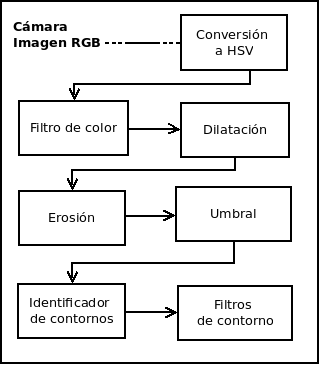
\includegraphics[scale=0.6]{vision/figures/vision-flow.png}
\end{center}
  \caption[Etapas del algoritmo de visi\'on]{Etapas del algoritmo de visi\'on}
  \label{fig:alg_steps}
\end{figure}


\subsubsection{\label{sec:color} Detecci\'on de color}
El problema de decidir si un pixel determinado se corresponde con un 
color particular resulta mucho m\'as sencillo de resolver en el espacio 
de color HSV que en el RGB. Este espacio de color se compone de un canal H que 
describe el color de un pixel, un canal S que pondera la saturaci\'on de 
dicho color y un canal V que mide la luminosidad de dicho pixel. En el espacio RGB, de haber un cambio en el brillo o 
iluminaci\'on de la imagen, los tres canales se ven afectados de igual 
manera mientras que en el espacio HSV el canal H, que codifica la 
informaci\'on sobre el tono del color, se ve mucho menos influenciado en 
comparaci\'on con los otros dos canales (saturaci\'on y valor). De esta 
manera, podemos caracterizar el color de un pixel determinado 
observando su valor en el canal H, sin molestarnos demasiado por las condiciones de brillo o iluminaci\'on al cual se encuentra expuesto.
\\ \indent Realizamos la detecci\'on de color verificando los valores 
correspondientes al canal H (tono) de la representaci\'on HSV de la 
imagen. Para esto convertimos de la imagen obtenida por la c\'amara  de formato RGB a HSV usando el algoritmo expuesto en la figura \ref{code:hsv}.
\begin{figure}[tpb]
\begin{verbatim}
V=max(R, G, B)
S=(V-min(R,G,B))*255/V   if V!=0, 0 otherwise

       (G - B)*60/S,  if V=R
H= 180+(B - R)*60/S,  if V=G
   240+(R - G)*60/S,  if V=B

if H<0 then H=H+360
\end{verbatim}
\caption[Conversión RGB-HSV]{\label{code:hsv}pseudo-c\'odigo de la conversi\'on RGB-HSV}
\end{figure}

Obteniendo el canal H, nos fijamos que los valores de los pixeles 
est\'en dentro de cierto rango correspondiente al color que buscamos. 
Como podemos observar en la figura \ref{fig:hsv_space}, en el espacio 
de color HSV los colores se encuentran dispuestos a lo largo de una 
circunferencia, donde cada tonalidad representa un \'angulo en la misma. 
Por ejemplo, si queremos abarcar las distintas tonalidades del azul 
podemos elegir el rango que va de 200$^\circ$ a 260$^\circ$. Cuando 
buscamos un color en particular  es preciso elegir este rango 
cuidadosamente ya que de ser un rango muy restrictivo podemos 
despreciar pixeles de inter\'es arruinando la figura del contorno del 
objeto a buscar y si elegimos un rango m\'as abarcativo podemos tomar 
pixeles de colores distintos al buscado, introduciendo ruido. 
Experimentalmente comprobamos los resultados de un filtro de color con 
distintos rangos, como se muestra  en la figura \ref{fig:hue_range}. 
Una vez obtenidos los pixeles que se corresponden con el color buscado 
se combinan estos con los del canal de saturaci\'on utilizando un and 
bit a bit entre ambos pixeles. A mayor saturaci\'on consideramos mayor 
presencia del color buscado en dicho pixel y por lo tanto mayor 
probabilidad de que \'este corresponda al objeto buscado. \\
\indent En el caso de las colillas se utiliz\'o el rango para el canal de tono 
$20<h<40$ con valor en el canal de saturaci\'on mayor a 60. En el caso 
de los platos y los vasos se busco detectar el color blanco. La 
particularidad de este color es que este se encuentra presente en 
todos los colores del rango H y se lo caracteriza por su valor alto en 
el canal $V$. Por este motivo, para platos y vasos s\'olo se verifica que 
se cumpla que el valor del pixel tenga $v>170$.
\begin{figure}[tpb]
\begin{center}
  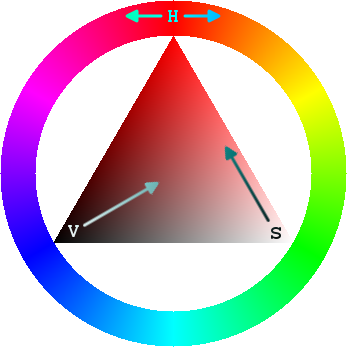
\includegraphics[scale=0.4]{vision/figures/hsv_triangle.png}
\end{center}
  \caption[Espacio de color HSV]{\small Espacio de color HSV. Los distintos tonos de colores se encuentran dispuestos a lo largo de la circunferencia.}
  \label{fig:hsv_space}
\end{figure}

\begin{figure}[tpb]
\begin{center}
  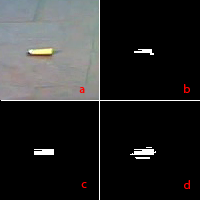
\includegraphics[scale=0.8]{vision/figures/hue.png}
\end{center}
  \caption[Filtro de color con distintos rangos]{\small Resultados de aplicar un filtro de color utilizando distintos rangos. (a) Captura original. (b) Resultado de aplicar el filtro $35\le h \le45$, se pierden algunos pixeles. (c) Resultado de aplicar el filtro $20\le h \le40$. (d) Resultado de aplicar el filtro $10 \le h \le 50$, se introducen pixeles extra.} 
  \label{fig:hue_range}
\end{figure}

	\subsubsection{\label{sec:thresh} Threshold}
Threshold o umbral es una operaci\'on que nos permite pasar de una 
imagen en escala de grises a una imagen binaria. El proceso de 
thresholding consiste en distinguir los pixeles que se encuentran por 
encima de un cierto valor de los que est\'an por debajo del mismo. Con 
este objetivo, se crea una imagen binaria asign\'andoles valores 1 o 0 
seg\'un su condici\'on respecto del valor. El algoritmo de thresholding 
nos puede servir para distinguir un objeto determinado de un contexto o 
fondo siempre y cuando el objeto posea un mayor brillo que el fondo en 
el que se encuentra. Ésto significa que los pixeles correspondientes a 
un objeto se encontrar\'an por encima de cierto valor caracter\'istico, 
determinado por el fondo. En nuestro caso \'esto no sucede de \'esta forma ya que no siempre la intensidad o brillo de los objetos supera al fondo en el que se encuentra, por lo cual resulta dif\'icil utilizar esta t\'ecnica. Podemos apreciar un ejemplo de este efecto en la figura \ref{fig:thresh-dif}. \\
\indent Existen diversas variantes de threshold, los par\'ametros 
utilizados son $Val$ para indicar el valor umbral y $M$ que indica el 
valor a tomar por los pixeles.
\begin{itemize}
\item{ Threshold binario:  Si un pixel se encuentra por encima de $Val$, se le asigna un valor $M$, de otro modo se le asigna $0$.}
\item{ Threshold binario invertido:  Si un pixel se encuentra por encima de $Val$, se le asigna 0, de otro modo se le asigna $M$.}
\item{ Threshold truncado:  Si un pixel se encuentra por encima de $Val$, se le asigna $V$, de otro modo conserva su valor.}
\item{ Threshold a cero invertido : Si un pixel se encuentra por encima de $Val$ se le asigna $0$, de otro modo, conserva su valor.}
\item{ Threshold a cero invertido : Si un pixel se encuentra por encima de $Val$ conserva su valor, de otro modo se le asigna $0$.}
\end{itemize}
El problema con esta familia de algoritmos es que en todos los casos el 
valor $Val$ permanece constante para toda la imagen haci\'endolo propenso 
a errores cuando la imagen presenta diferentes niveles de iluminaci\'on. 
Una manera de solucionar esto es pre-computando el valor $Val$ para 
distintas zonas de la imagen como lo hace la 
t\'ecnica de thresholding adaptativo, que computa el valor de $Val$ a 
medida que recorre la imagen, usando para esto, una ventana cuyo 
tama\~no es definido por el usuario. Siguiendo esta l\'ogica, se utilizan 
los valores de los pixeles abarcado por esta ventana para definir un valor 
de $Val$ (por ejemplo calculando el promedio de intensidad) y luego se 
aplica alguna de las t\'ecnicas de thresholding simples mencionadas, 
utilizando este mismo valor. Sin embargo, este algoritmo es m\'as 
costoso y puede provocar efectos indeseados como se observa en la 
figura \ref{fig:thresh_adapt} en donde el valor de $Val$ se calcula 
utilizando un promedio ponderado por una funci\'on gausseana de acuerdo a la distancia del centro 
de la ventana.\\
\indent En nuestro caso, utilizamos thresholding no para distinguir los 
objetos del fondo (esto es trabajo del filtro de color), sino como 
m\'etodo de eliminaci\'on de ruido. Cuando se combina el canal de 
saturaci\'on con el resultado del filtro de color, se obtiene una imagen 
de escala de grises que esta segmentada en un conjunto de \'areas con 
distintos valores de intensidad. Luego de aplicar dilataci\'on y 
erosi\'on, los niveles de intensidad de cada \'area se vuelven 
homog\'eneos (ya que se toma el m\'aximo o m\'inimo local) y es entonces 
donde podemos diferenciar las zonas de intensidad alta de las zonas de 
intensidad baja, motivo por el cual utilizamos la operaci\'on de 
threshold. En las figuras \ref{fig:threshold_ruido} y 
\ref{fig:threshold} exhibimos dos casos de ejemplo de threshold. 
Para la detecci\'on de colillas, vasos y platos establecemos 
el umbral de la operaci\'on de threshold en $100$, asign\'andoles un valor 
de $255$ (valor m\'aximo) a los pixeles que superen dicho umbral o $0$ en 
caso en contrario. Podemos apreciar un ejemplo de threshold en la 
figura \ref{fig:threshold}.

\begin{figure}[tpb]
\begin{center}
  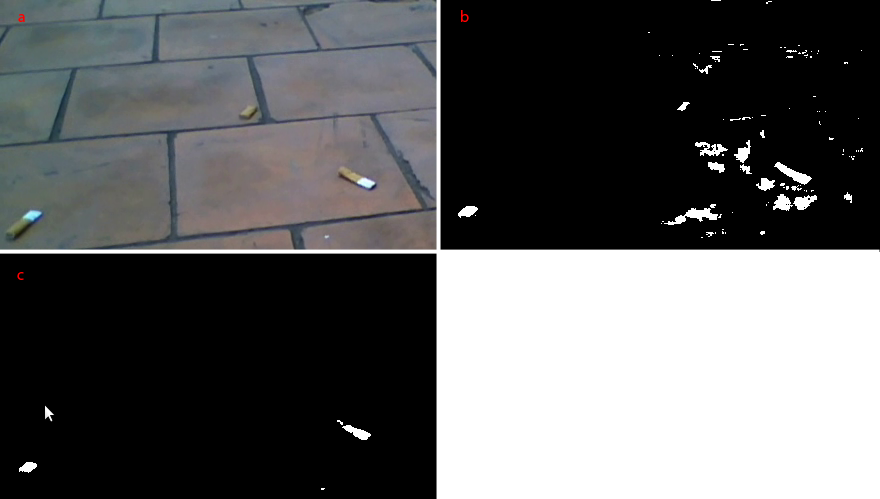
\includegraphics[scale=0.4]{vision/figures/threshold-dif.png}
\end{center}
  \caption[Distintos valores de umbral]{\small Distintos valores de umbral. (a) Captura original. 
  (b) Threshold binario con umbral 120. Se observan pixeles extra en 
  la detecci\'on. (c) Threshold binario con umbral 160. Se observa la 
  ausencia de pixeles. }
  \label{fig:thresh-dif}
\end{figure}

\begin{figure}[tpb]
\begin{center}
  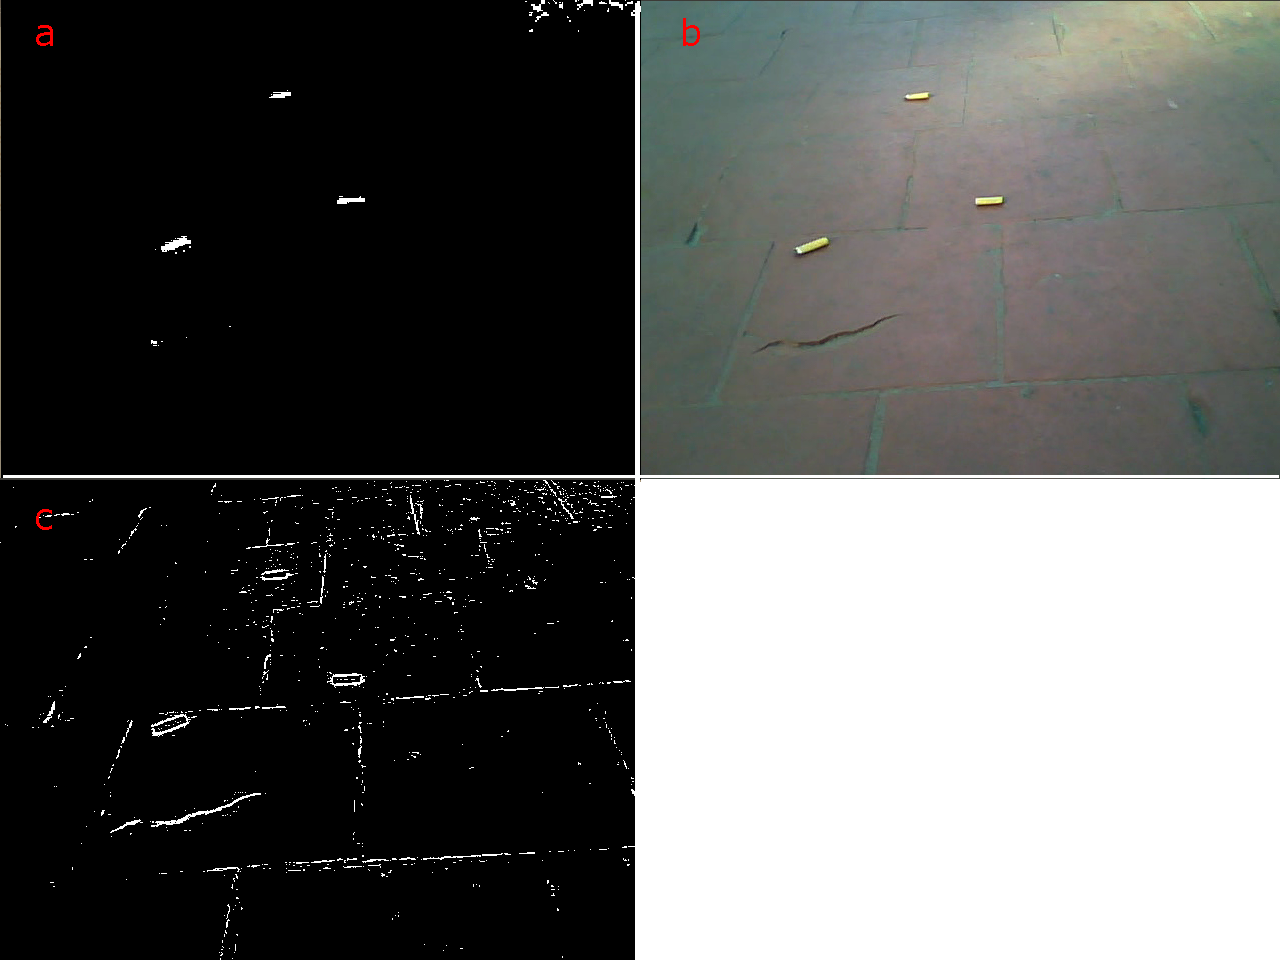
\includegraphics[scale=0.25]{vision/figures/adaptative.png}
\end{center}
  \caption[Comparación threshold con filtro de color]{\small Comparaci\'on de threshold adaptativo con el filtro de 
  color. (b) Imagen obtenida de la c\'amara. 
  (a) Salida del filtro de color. (c) Threshold adaptativo sobre la 
  imagen b previa conversi\'on a blanco y negro utilizando una ventana 
  de 9x9 pixeles. Se observa que el filtro adaptativo identifica 
  correctamente los contornos de las colillas pero agrega mucha 
  informaci\'on redundante que resultara en procesamiento extra.}
  \label{fig:thresh_adapt}
\end{figure}


\begin{figure}[tpb]
\begin{center}
  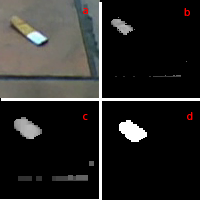
\includegraphics[scale=0.8]{vision/figures/threshold-ruido.png}
\end{center}
 \caption[Eliminación de ruido por threshold]{\small Resultados de aplicar thresholding binario. (a) Captura original. (b) Salida del detector de color, se observan algunos pixeles extra cerca de la l\'inea de brea. (c) Salida de la operaci\'on de dilataci\'on-erosi\'on. (d) Salida de la operaci\'on de thresholding binario con un umbral de $100$. La baja intensidad de los pixeles extra en la l\'inea de brea no supera el umbral propuesto y por lo tanto son descartados. El contorno del objeto de inter\'es se conserva aislado.} 
  \label{fig:threshold_ruido}
\end{figure}

\begin{figure}[tpb]
\begin{center}
  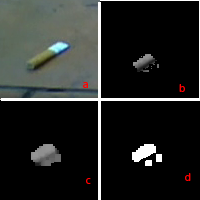
\includegraphics[scale=0.8]{vision/figures/threshold.png}
\end{center}
  \caption[Resultados de aplicar thresholding]{\small Resultados de aplicar thresholding. (a) Captura original. (b) Salida del detector de color, se observan algunos pixeles extra debajo del objeto de inter\'es. (c) Salida de la operaci\'on de dilataci\'on-erosi\'on, los pixeles extra se combinaron con los pixeles del objeto.(d) Salida de la operaci\'on de thresholding binario con un umbral de $100$. La baja intensidad de los pixeles extra en la zona debajo del objeto no supera el umbral propuesto y por lo tanto son descartados. El contorno del objeto de inter\'es se conserva aislado.} 
  \label{fig:threshold}
\end{figure}

	\subsubsection{\label{sec:morph} Operaciones morfol\'ogicas}
Sombras, luces y otros efectos pueden alterar el resultado del filtro 
de color introduciendo ruido en los objetos a detectar. Este ruido 
puede surgir tanto de la omisi\'on de pixeles de inter\'es como  inclusi\'on de pixeles extra. Para subsanar esto, utilizamos las operaciones morfol\'ogicas de dilataci\'on y erosi\'on. Ambas se basan en la utilizaci\'on de un elemento estructural, esto es, una figura de cualquier tama\~no y forma que tiene definido un punto principal y que recorre la imagen solap\'andose pixel a pixel. De acuerdo a operaciones locales a este elemento, el pixel que coincide con el punto principal se ve modificado. Usualmente se utilizan como elementos estructurales, peque\~nos discos o cuadrados, donde el punto principal se encuentra en el centro del mismo. El efecto generado se entiende mejor observ\'andolo en im\'agenes binarias. En el caso de la dilataci\'on, la idea intuitiva es remplazar cada pixel no vac\'io con una copia del elemento estructural cuyo punto principal se encuentra en esa posici\'on. Para la erosi\'on, la idea intuitiva es quedarse con aquellos pixeles tal que podamos hacer caber un elemento estructural cuyo punto principal se encuentra en esa posici\'on y dicho elemento solo cubra pixeles no vac\'ios.
Ilustramos esto en las figuras \ref{fig:dilate-sample} y \ref{fig:erode-sample}.


\begin{figure}[tpb]
\begin{center}
  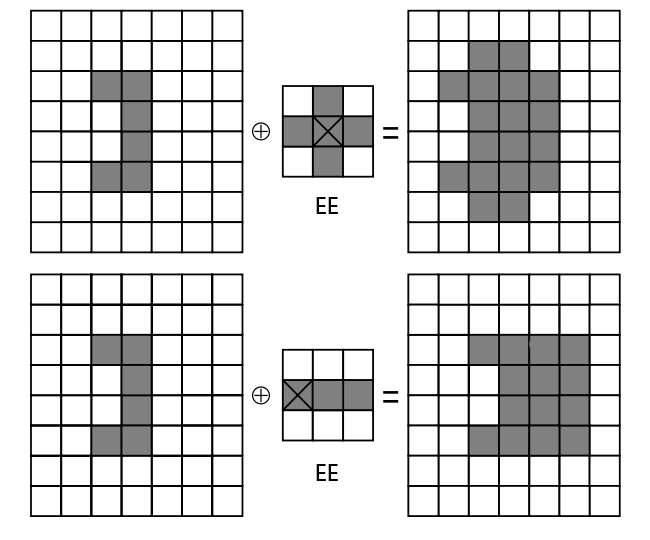
\includegraphics[scale=0.4]{vision/figures/dilate-sample.png}
\end{center}
  \caption[Operaci\'on de dilataci\'on]{\small Operaci\'on de dilataci\'on en im\'agenes binarias. Se reemplazan los pixeles no vac\'ios por una copia del elemento estructural con punto principal en esa posici\'on. La cruz indica la posici\'on del punto principal dentro del elemento estructural (ee). Imagen obtenida del curso de visi\'on artificial de la Universidad Polit\'ecnica de Madrid.}
  \label{fig:dilate-sample}
\end{figure}

\begin{figure}[tpb]
\begin{center}
  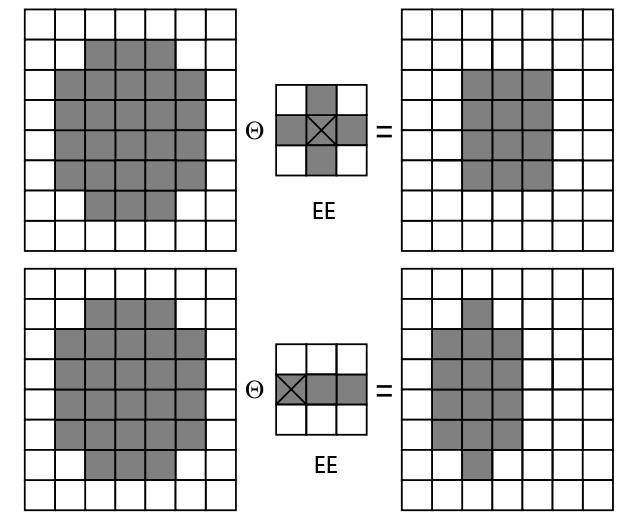
\includegraphics[scale=0.4]{vision/figures/erode-sample.png}
\end{center}
  \caption[Operaci\'on de erosi\'on]{\small Operaci\'on de erosi\'on en im\'agenes binarias. Se persisten los pixeles no vac\'ios en donde cabe una copia del elemento estructural cuyo punto principal se encuentra en esa posici\'on. La cruz indica la posici\'on del punto principal dentro del elemento estructural (ee). Imagen obtenida del curso de visi\'on artificial de la Universidad Polit\'ecnica de Madrid. } 
  \label{fig:erode-sample}
\end{figure}

	\paragraph{Dilataci\'on}
En im\'agenes no binarias, la operaci\'on de dilataci\'on se define 
tomando el m\'aximo local bajo el elemento estructural y asign\'andole ese valor al punto principal. El efecto producido es una reducci\'on general en el brillo de la imagen y un probable aumento el tama\~no de las figuras \cite{nasa-dilate-erode}.  Cuando un \'area grande aparece, a causa del ruido, partida en varias componentes, el uso de la operaci\'on de dilataci\'on provoca que  se combinen nuevamente en una sola. Un ejemplo de esto puede ser apreciado en la figura \ref{fig:dilate}. Otro beneficio de utilizar dilataci\'on es la eliminaci\'on del ruido espurio como se aprecia en la figura \ref{fig:dilate-ruido}.

\begin{figure}[tpb]
\begin{center}
  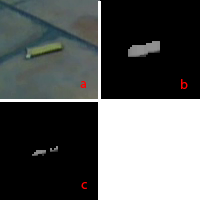
\includegraphics[scale=0.8]{vision/figures/dilate1.png}
\end{center}
  \caption[Efecto de la operaci\'on de dilataci\'on]{\small Efecto de la operaci\'on de dilataci\'on. (a)  Imagen original tomada de la c\'amara. (b) Imagen luego de aplicar dilataci\'on a la imagen c con un elemento estructural cuadrado de 3x3 pixeles, con punto principal en el centro. (c) Salida del filtro de color. La colilla de cigarrillo esta 'partida' en dos componentes conexas. } 
  \label{fig:dilate}
\end{figure}

\begin{figure}[tpb]
\begin{center}

  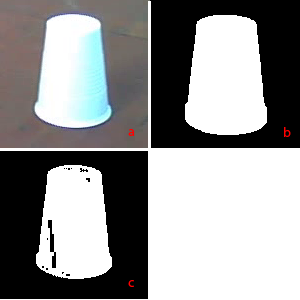
\includegraphics[scale=0.6]{vision/figures/dilate-ruido.png}
\end{center}
  \caption[Eliminaci\'on de ruido mediante dilataci\'on]{\small Eliminaci\'on de ruido mediante la operaci\'on de dilataci\'on. (a) Imagen original tomada de la c\'amara. (b) Imagen luego de aplicar dilataci\'on a la imagen c con un elemento estructural cuadrado de 3x3 pixeles, con punto principal en el centro. (c) Salida del filtro de color. Observamos \'areas  oscuras en el interior del vaso. }
  \label{fig:dilate-ruido}
\end{figure}

	\paragraph{Erosi\'on}
En im\'agenes no binarias, la operaci\'on de erosi\'on se define tomando el m\'inimo local bajo el elemento estructural y poni\'endole ese valor al punto principal. Contrario a la dilataci\'on, este operador generalmente reduce el brillo de la imagen y disminuye el tama\~no de las figuras \cite{nasa-dilate-erode}. Usamos la operaci\'on de erosi\'on para eliminar las protuberancias que pueden surgir de aplicar la operaci\'on de dilataci\'on. En la figura \ref{fig:erode} podemos apreciar el efecto de aplicar dilataci\'on y luego erosi\'on.

\begin{figure}[tpb]
\begin{center}
  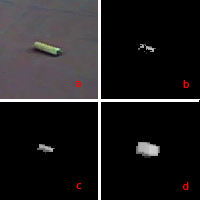
\includegraphics[scale=0.8]{vision/figures/erosion.png}
\end{center}
  \caption[Ejemplo de erosi\'on]{\small Ejemplo de erosi\'on. (a) Captura original. (b) Salida del filtro de color. Se observan fallas en la detecci\'on del objeto. (d) Se aplica la operaci\'on de dilataci\'on a la imagen b. Se observa la producci\'on de protuberancias en la figura del objeto. (c) Salida luego de aplicar erosi\'on a c. La figura del objeto se corrige eliminando parte de las protuberancias. Sin embargo, no se observan fallas en la detecci\'on del objeto. }
  \label{fig:erode}
\end{figure}

	\subsubsection{Detecci\'on de contornos}
	La detecci\'on de contornos se realiza sobre las im\'agenes binarias producidas en la etapa de pre-procesamiento. Dichos contornos
	quedan definidos impl\'icitamente como la separaci\'on de regiones 
	positivas de las negativas \footnote{ Como se trata de im\'agenes 
	binarias, llamamos a una regi\'on positiva a las que contienen 
	pixeles con valores mayores a 0 y a las negativas a las que tienen 
	un valor de 0.}. Por lo tanto para obtener estas regiones hacemos 
	uso de los algoritmos explicados en esta sub-secci\'on.
	
	\paragraph{Algoritmo} 
	Recordemos que las im\'agenes binarias se caracterizan por tener solo 
	dos tipos de pixeles, los que tienen un valor de $0$ y los que tienen 
	un valor mayor a 0. Denominamos a estos pixeles como 
	0-pixeles o 1-pixeles respectivamente. Decimos que un conjunto de 
	0-pixeles o 1-pixeles \textit{conectados} forman una componente. Entendemos dos tipos de conectividad:
	la 4-conectividad y la 8-conectividad. Dos pixeles con coordenadas 
	$(x',y')$ y $(x'',y'')$ son 4-conexos si y s\'olo si 
	$|x' - x''| + |y'-y''| = 1$ y 8-conexos si y s\'olo si $max(|x'-x''|,|y'-y''|)=1$, la figura \ref{fig:conectividad} ilustra estas relaciones.
	Usando este concepto de conectividad se puede segmentar una imagen 
	binaria en varias componentes 4-conexas u 8-conexas formadas por 
	 0-pixeles o 1-pixeles. Cada una de estas
	componentes se compone de pixeles de valores iguales y, para cualquier 
	par de pixeles pertenecientes a la componente, existe un 
	4-camino u 8-camino \footnote{ Un 4-camino u 8-camino, es una secuencia 
	de pixeles tal que cada pixel es 4-conexo u 8-conexo con el pixel 
	siguiente.} que los
	conecta. Ya que las 1-componentes (componentes que contienen 
	1-pixeles) son complementarias con las 0-componentes podemos s\'olo considerar las primeras y asumir que todo
	lo dem\'as corresponde a 0-pixels conformando el fondo de la imagen. Cada 
	1-componente posee un \'unico borde exterior que lo separa de la 0-componente que lo rodea y cero o m\'as bordes interiores que lo separan de las 0-componentes que rodea (agujeros). Un ejemplo de esto puede apreciarse
	en la figura \ref{fig:contours}. El algoritmo que utilizamos no tiene 
	en cuenta agujeros interiores de un contorno. Definimos entonces un 
	punto de borde a un elemento de una 1-componente que es 4-conexo con 
	una 0-componente y al \textit{borde} o \textit{contorno} de una figura 
	como un conjunto de puntos de borde conectados.\\
	\indent El objetivo de este algoritmo es entonces recolectar todos los 
	puntos de la imagen caracterizados como puntos de borde. Para 
	hacer esto, recorre la imagen l\'inea por l\'inea buscando nuevos puntos de borde, cuando encuentra
	uno nuevo, activa un proceso de seguimiento de borde almacenando las 
	coordenadas de cada punto que lo compone. Durante este proceso va 
	marcando los pixeles ya 
	visitados asign\'andoles a estos un valor especial para no volver a 
	incidir en ellos. Finalmente se disponen todos los contornos encontrados en una lista.
	Este algoritmo de reconocimiento de contornos est\'a basado en la 
	t\'ecnica expuesta por Suzuki y Abe (para mayor detalle referimos al 
	autor a \cite{suzuki85}).
	
	\begin{figure}[tpb]
\begin{center}
  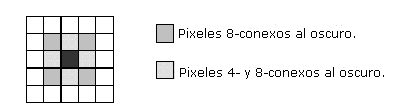
\includegraphics[scale=0.6]{vision/figures/48conexos.png}
\end{center}
  \caption[Tipos de conectividad entre pixeles]{\small Tipos de conectividad entre pixeles de una imagen binaria}
  \label{fig:conectividad}
\end{figure}

\begin{figure}[tpb]
\begin{center}
  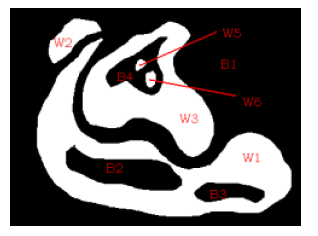
\includegraphics[scale=0.6]{vision/figures/zonas-contours.png}
\end{center}
  \caption[Ejemplo de segmentaci\'on en im\'agenes binarias]{\small Ejemplo de segmentaci\'on en im\'agenes binarias. Las 1-componentes w1,w2 y w3 se encuentran rodeadas por la componente de fondo b1 y a su vez
  rodean a 0-componentes b2, b3 y b4 }
  \label{fig:contours}
\end{figure}
	
	
	\paragraph{Representaci\'on}
	Como se expresa en el trabajo de Zhang y Lu \cite{Zhang02}, existen diversas formas de representar los contornos, cada una con
	distintas aplicaciones. En nuestro caso utilizamos la codificaci\'on 
	encadenada de Freeman, que consiste en describir una sucesi\'on de puntos
	de acuerdo a la posici\'on de un punto con respecto a su predecesor en 
	la secuencia. Para lograr esto se numeran los vecinos de un pixel con 
	los n\'umeros del 0 al 7 como indica la figura \ref{fig:freeman}. As\'i un contorno puede almacenarse como la coordenada de
	un punto inicial seguido de una cadena de c\'odigos (del 0 al 7) que indican la posici\'on del pr\'oximo punto respecto al actual. Esta 
	es una representaci\'on m\'as compacta en comparaci\'on con una secuencia 
	de coordenadas  $(x,y)$ y posibilita la extracci\'on de 
	caracter\'isticas tales como el CCH o NCCH \footnote{ CCH o chain 
	code histogram es un histograma que se extrae a partir de la 
	frecuencia de aparici\'on de los n\'umeros 0 a 7 en un contorno 
	codificado con cadenas de Freeman. Este descriptor es invariante 
	frente a traslaciones y escalamientos pero no frente a rotaciones 
	para lo que existe su versi\'on normalizada NCCH. Para m\'as detalle 
	ver \cite{Iivarinen96shaperecognition}}. La figura \ref{fig:freeman_sample} exhibe un 
	ejemplo de codificaci\'on utilizando este m\'etodo.
	
	\begin{figure}[htpb]
\begin{center}
  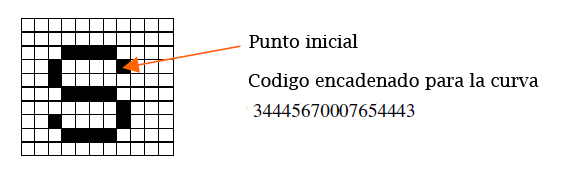
\includegraphics[scale=0.6]{vision/figures/freeman-sample.png}
\end{center}	
  \caption[Ejemplo de codificaci\'on de un contorno utilizando los c\'odigos de Freeman]
  {\small Ejemplo de codificaci\'on de un contorno utilizando los c\'odigos de Freeman. }
  \label{fig:freeman_sample}
\end{figure}

\begin{figure}[htpb]
\begin{center}
  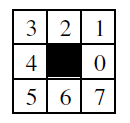
\includegraphics[scale=0.6]{vision/figures/freeman-codes.png}
\end{center}
  \caption[Matriz para la codificaci\'on de Freeman]{\small Matriz para la codificaci\'on de Freeman. El n\'umero indica la direcci\'on de desplazamiento del pr\'oximo punto respecto del
  actual (punto negro) }
  \label{fig:freeman}
\end{figure}
		
		
	\paragraph{Pol\'igonos}
	Como mencionamos, los contornos son representados utilizando la codificaci\'on de Freeman. Sin embargo, la precisi\'on con la que se muestrean estos bordes suele ser excesiva o redundante para nuestras
	necesidades lo cual hace el an\'alisis de figuras m\'as dif\'icil. Con el fin de reducir esta complejidad utilizamos un algoritmo
	para representar el mismo contorno con una menor cantidad de puntos. Esto se realiza mediante un algoritmo de aproximaci\'on por pol\'igonos
	basado en el trabajo de Douglas y Pecker \cite{dp74}. Previo a la aplicaci\'on de este algoritmo, convertimos el contorno a una representaci\'on
	tradicional de secuencias de puntos $(x,y)$ correspondientes a las 
	coordenadas del borde en la imagen. Esto se puede lograr f\'acilmente partiendo del punto inicial y calculando la variaci\'on en la coordenada seg\'un el c\'odigo de vecino correspondiente ( 0-7).\\
	\indent La t\'ecnica de aproximaci\'on comienza tomando los dos puntos 
	pertenecientes al contorno m\'as alejados entre s\'i. Estos puntos se 
	agregan a la aproximaci\'on y se traza una l\'inea entre ellos.
	Luego se recorre el resto de los puntos del contorno buscando a aquel 
	que se encuentre a mayor distancia de esta l\'inea. A dicho punto se lo 
	agrega a la aproximaci\'on, generando dos nuevas l\'ineas con los dos puntos iniciales. Este proceso se itera agregando siempre el punto que se encuentre m\'as distante de la aproximaci\'on hasta que todos los puntos del contorno se encuentren a una distancia menor que cierto par\'ametro 
	de precisi\'on establecido. En la figura \ref{fig:polyaprox} podemos 
	apreciar una esquematizaci\'on de este proceso.\\
	\indent Otra ventaja que 
	otorga la utilizaci\'on de esta aproximaci\'on es que si un contorno 
	presenta una serie de puntos alineados, estos ser\'an remplazados por 
	un \'unico segmento o lado del pol\'igono, lo que nos permite 
	identificar l\'ineas en los contornos. Esta caracter\'istica es 
	aprovechada para realizar la detecci\'on de vasos como se ve en la  
	secci\'on \ref{sec:filtros}. En la figura \ref{fig:polyVasos} podemos observar un contorno
	y su aproximaci\'on por pol\'igonos.
	
\begin{figure}[htpb]
\begin{center}
  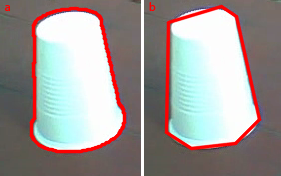
\includegraphics[scale=0.8]{vision/figures/polyaprox.png}
\end{center}
  \caption[Aproximaci\'on de contornos mediante pol\'igonos]{\small Aproximaci\'on de contornos mediante pol\'igonos. (a) Se observa que el contorno se encuentra acorde el borde del vaso, las
  partes laterales del mismo se encuentran segmentadas (efecto serrucho) por la cantidad de puntos. (b) El contorno es representado mediante
  8 puntos, los lados laterales solo involucran un segmento posibilitando la detecci\'on de l\'ineas.}
  \label{fig:polyVasos}
\end{figure}

\begin{figure}[htpb]
\begin{center}
  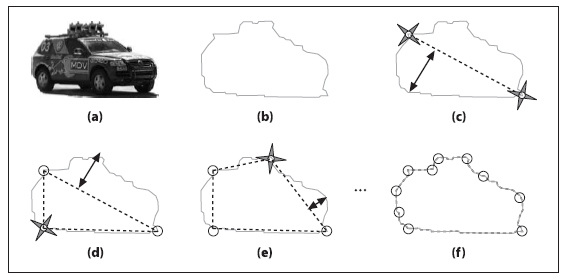
\includegraphics[scale=0.6]{vision/figures/douglas-pecker.png}
\end{center}
  \caption[Algoritmo de aproximaci\'on de pol\'igonos]{\small Iteraciones del algoritmo de aproximaci\'on de pol\'igonos de Douglas-Peucker. (a) Imagen original. (b) Extracci\'on de contorno
  (c) Se seleccionan dos puntos iniciales y se traza una l\'inea entre ellos (d) Se agrega a la aproximaci\'on el punto m\'as lejano del contorno a esta l\'inea.
  (e) Se repite el proceso agregando siempre el punto m\'as lejano (f) hasta que todos los puntos est\'en a cierta distancia requerida.}
  \label{fig:polyaprox}
\end{figure}

	

	\subsubsection{\label{sec:filtros} Filtros}
	Realizada la etapa de pre-procesamiento y la recolecci\'on de contornos 
	de la imagen, el paso que sigue es verificar que estos
	contornos tengan caracter\'isticas que correspondan con  los 
	objetos buscados. Para realizar esto, se implementan una serie de filtros que verifican propiedades
	puntuales sobre los mismos de forma tal que, si un contorno supera todos los filtros entonces consideramos a tal como un objeto reconocido. \\
	\indent Los filtros se disponen en cascada, es decir, se prueba un 
	filtro en un contorno si y s\'olo si este super\'o todos los filtros 
	anteriores. De esta forma podemos ordenar los filtros de m\'as general 
	a m\'as espec\'ifico, optimizando (generalmente) los tiempos de detecci\'on. Por ejemplo, conocer 
	el \'area que abarca un contorno determina f\'acil y r\'apidamente si un contorno corresponde a una colilla o a un plato evitando la ejecuci\'on
	de filtros m\'as espec\'ificos. En la figura \ref{fig:desc} se exhiben 
	los valores obtenidos por algunos de los filtros que detallamos a 
	continuaci\'on:
	\paragraph{Filtro de \'area}
	El filtro de \'area calcula el \'area encerrada por un contorno y verifica que la misma se encuentre por encima y/o por debajo
	de valores determinados. El \'area encerrada por un contorno se computa utilizando la formula de Green \cite{greenwolfram}.
	Si bien esto es m\'as veloz que contabilizar todos los pixeles encerrados en el contorno, posee la desventaja que no se tienen en cuenta agujeros
	en el interior del mismo.
	\paragraph{Filtro de \'area por zona}
	Un objeto que posee un \'area determinada puede ocupar m\'as o menos pixeles dependiendo de su ubicaci\'on en la imagen. Este se debe a la 
	perspectiva de la c\'amara y puede afectar al reconocimiento de un contorno. Para contemplar esta variaci\'on se pueden establecer distintas
	zonas en la imagen y definir distintos valores de \'area m\'inimos y m\'aximo para cada una de ellas. Al ejecutarse este filtro se calcula la
	zona a la cual pertenece dependiendo de su ubicaci\'on en la imagen y se verifican los valores para dicha zona, si este los satisface entonces
	el contorno supera al filtro.
	\paragraph{Filtro de per\'imetro}
	El filtro de per\'imetro calcula, efectivamente, el per\'imetro 
	cubierto por un contorno . Esto se hace contando la cantidad de pixeles que lo definen.
	Vale remarcar, que el valor del per\'imetro depende ampliamente de la precisi\'on con la que se obtengan los bordes ya que se ve dr\'asticamente modificado 
	si se aumenta o disminuye dicha precisi\'on.
	\paragraph{Filtro de excentricidad}
	La excentricidad es un par\'ametro que relaciona la longitud del eje 
	m\'as largo con la del m\'as corto. Esta se define como 
	\textit { longitud del eje m\'as largo / longitud del eje m\'as corto}  . Algunas figuras pueden caracterizarse por tener valores de excentricidad
	que se mantienen en cierto rango y permite identificarlas usando este filtro.
	\paragraph{Filtro de circularidad}
	La circularidad es un par\'ametro que relaciona \'area con per\'imetro y define la redondez de una figura. Se define como $perimetro^2/area$. Algunas figuras pueden 
	caracterizarse por tener valores de circularidad que se mantienen en cierto rango y permite identificarlas usando este filtro.
	\paragraph{Filtro de \'area rectangular}
	El filtro de \'area rectangular relaciona el \'area del objeto con el \'area del rect\'angulo contenedor m\'inimo. Este verifica que el \'area
	del contorno cubra en gran parte el \'area del rect\'angulo. Esto se logra mediante la divisi\'on $(area contorno / area rectangulo)> p$, donde 
	$p$ es el porcentaje de \'area que queremos que sea cubierto.
	\paragraph{Filtro de elipse}
	El filtro de elipse verifica que un contorno determinado se ajuste o no a una elipse. Esto se logra usando un algoritmo basado 
	en cuadrados m\'inimos. El mismo retorna como resultado las longitudes de los semi-ejes de la elipse $a$ y $b$. Con estas medidas calculamos
	el \'area seg\'un la f\'ormula $A=\pi a  b$ y se la compara con la 
	obtenida a trav\'es del filtro de \'area. Se computa como $|A-AReal|/ 
	AReal < p$ donde p determina el
	valor de verosimilitud. Un valor de $p$ mas chico significa mayor 
	semejanza con una elipse. Si estas dos \'areas son lo suficientemente similares consideramos que el contorno supera el filtro. 
	Para el ajuste de elipse se utiliza el algoritmo Fitzgibbon, Pilu y Fisher \cite{Fitzgibbon99}.
	\paragraph{Filtro de vaso}
	El filtro para vasos consiste en varias etapas. Recordando que el contorno se codifica como un pol\'igono, se obtienen los dos segmentos 
	m\'as largos y se verifica que estos no compartan v\'ertices. Por otro lado se pide que la suma de la longitud de estos dos segmentos supere al $50\%$ del 
	per\'imetro del contorno, indicado por dicho filtro. Finalmente, se verifica que la distancia m\'inima entre estos dos ejes sea mayor a cierto valor prefijado, proporcional a la
	longitud del segmento m\'as largo. El filtro se basa en la idea de que 
	los dos segmentos m\'as largos se correspondan con los lados laterales 
	del vaso.  Se puede apreciar una foto  de un contorno que ha 
	verificado este filtro en la figura \ref{fig:polyVasos}. 
	\paragraph{Filtro de histograma}
	El filtro de histograma verifica la similitud de un histograma obtenido a partir del contorno con otro histograma obtenido a partir de 
	una imagen modelo del objeto a detectar. El histograma modelo se calcula en el inicio de la ejecuci\'on mientras que el del contorno se
	computa en tiempo real. Esto se hace obteniendo el rect\'angulo 
	contenedor m\'inimo de dicho contorno y computando un histograma 2D de la imagen
	utilizando los canales de saturaci\'on y tono. De esta manera, se 
	puede caracterizar a un objeto por una composici\'on de colores y no por su forma. El 
	problema de este filtro es que requiere mayor procesamiento.
	
	\subsubsection{Reconocimiento de vasos}
	Para el reconocimiento de vasos se utilizan(en este orden) los filtros de \'area, per\'imetro, circularidad y el de vasos.
	El filtro de \'area verifica que $500 \leq area \leq 10000 $, el de 
	per\'imetro que $100 \leq per \leq 800 $ y el de circularidad
	que $14 \leq circ \leq 18$. El filtro de vasos no es parametrizado. 
	
	\subsubsection{Reconocimiento de colillas}
	Para el reconocimiento de vasos se utilizan(en este orden) los filtros de \'area, per\'imetro y \'area rectangular.
	El filtro de \'area verifica que $50 \leq area \leq 800 $, el de per\'imetro que $10 \leq per \leq 150 $ y el de \'area rectangular
	que sea cubierto el $70\%$ del \'area del rect\'angulo contenedor m\'inimo.
	
	\subsubsection{Reconocimiento de platos}
	Para el reconocimiento de platos se utilizan(en este orden) los filtros de \'area, per\'imetro, circularidad, excentricidad y de elipse.
	El filtro de \'area verifica que $500 \leq area \leq 10000 $, el de per\'imetro que $500 \leq per \leq 1500 $, el de circularidad
	que $10 \leq circ \leq 16$, el de excentricidad que $0.65 \leq ecc \leq 0.95$ y el de elipse que $|a-aReal|/ aReal < 0.2$.
	
	\subsubsection{Centroide}
	El centroide es el centro geom\'etrico o centro de 
	gravedad de una figura y 
	sirve como punto de referencia para la misma. Para calcular dicho 
	punto hacemos uso de las formulas propuestas por Hu \cite{Hu1962} para la 
	descripci\'on de figuras. El momento de Hu de un contorno 2D se define como:
	\begin{equation}
		m_{pq}=\sum_{x}{\sum_{y}{x^py^qI(x,y)}}
	\end{equation}
	
	donde $I(x,y)$ es la intensidad del pixel de coordenadas $(x,y)$.
	Notamos que $m_{0,0}$ representa la suma de la intensidad de todos los pixeles del 
	contorno. Entonces, podemos definir al centroide $(x_c,y_c)$ como 
	$x_c= m_{1,0} / m_{0,0}$ e 
	$y_c=m_{0,1} / m_{0,0}$. Estas dos f\'ormulas se corresponden con el 
	promedio de las coordenadas x e y de los puntos de la figura.  


\begin{figure}[tpb]
\begin{center}
  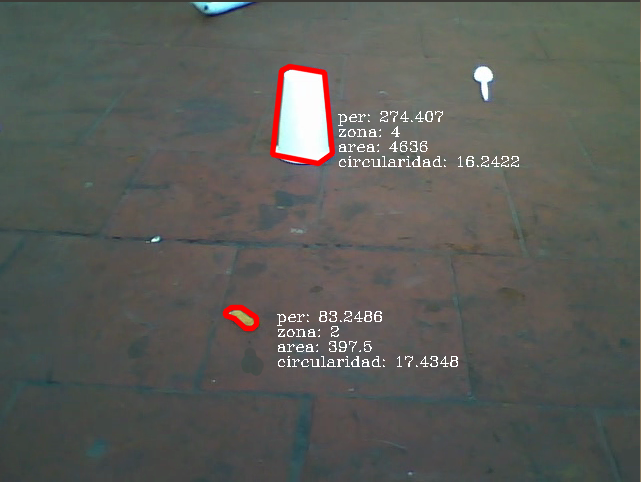
\includegraphics[scale=0.4]{vision/figures/filtros.png}
\end{center}
  \caption[Ejemplo de descriptores de contorno]{\small Ejemplo de descriptores de contorno. Se visualiza el \'area, per\'imetro, zona y circularidad del contorno 
  detectado de una colilla y un vaso}
  \label{fig:desc}
\end{figure}

	\subsection{Sistema de predicci\'on}
	El algoritmo de visi\'on que hemos descripto hasta aqu\'i funciona 
	procesando la imagen correspondiente a un \'unico cuadro. Sin embargo, 
	el sistema de visi\'on del robot debe permitir el reconocimiento de 
	objetos a medida que \'este se desplaza por su entorno y por lo tanto 
	dicho sistema debe procesar im\'agenes secuenciales del mismo. Con 
	esto afirmamos que existe cierta relaci\'on (tanto temporal como 
	espacial) entre las im\'agenes 
	que el sistema de visi\'on debe procesar y que podemos aprovechar esta 
	caracter\'istica para reforzar la detecci\'on de objetos. El mecanismo por el cual buscamos lograr este objetivo es el del sistema de predicci\'on.\\
\indent 	El sistema de predicci\'on consume la informaci\'on que el 
sistema de visi\'on le entrega en cada cuadro y, con ella, realiza el 
seguimiento de objetos a lo largo del tiempo. Es a partir de este 
seguimiento que el sistema de predicci\'on toma decisiones sobre la 
posici\'on o existencia de los objetos que el sistema de visi\'on 
reconoce. Vale destacar que estos dos sistemas pueden encontrarse, a 
menudo, en desacuerdo acerca de presencia u ausencia 
de un objeto.  El sistema de predicci\'on se basa en las siguientes asunciones:
\begin{enumerate}
\item{ Los objetos no realizaran grandes desplazamientos entre cuadros 
consecutivos - esto se debe a la proximidad temporal entre cuadros y que el robot no realiza movimientos bruscos.}
\item{ Los objetos no sufrir\'an grandes alteraciones en su forma, \'area 
o per\'imetro entre cuadros consecutivos - con un razonamiento similar, la perspectiva no cambia lo suficiente como para alterar la figura, \'area o per\'imetro de los objetos.}
\end{enumerate} 
Con estas premisas, dado un objeto $A$ reconocido en el cuadro $c_0$, 
cuyo centroide se encuentra en las coordenadas (en la imagen) $(x_0,y_0)$, \'area $a$ y per\'imetro $p$, 
el sistema de predicci\'on asume que si se encuentra un objeto $A'$ en 
el cuadro siguiente $c_1$ con coordenadas $(x_1, y_1)$ tal que 
$||(x_1,y_1) - (x_0,y_0)||\leq \alpha$, \'area $a'$ tal que $|a-a'| \leq 
\gamma *a$ y per\'imetro $p'$ tal que $|p-p'|\leq \theta*p$ entonces $A 
\simeq A'$, donde $\alpha$, $\gamma$ y $\theta$ son par\'ametros del 
sistema. Esta afirmaci\'on no solo vale para el cuadro subsiguiente 
$c_1$ sino tambi\'en para los siguientes $c_2,c_3 ... c_{0+\eta}$ donde 
$\eta$ y $\alpha$ se computan, para este caso, seg\'un el 
historial de detecci\'on de cada objeto.  Bas\'andose en esta regla, el 
sistema de predicci\'on puede estimar la posici\'on de un objeto que, 
para un cuadro en particular, no fue detectado por el sistema de 
visi\'on. Para concretar este mecanismo, cuando un objeto es detectado a lo largo de varios cuadros se persiste la siguiente informaci\'on:
\begin{itemize}
\item{ Última posici\'on, \'area y per\'imetro - Se toman los datos de la 
detecci\'on m\'as reciente del sistema de visi\'on.}
\item{ Antigüedad del objeto - Cantidad de cuadros transcurridos desde que se comenz\'o a persistir el objeto en el sistema de predicci\'on.}
\item{ Cantidad de detecciones - Se mantiene la cantidad de cuadros en la cual el sistema de visi\'on detect\'o al objeto.}
\item{ Desplazamiento en la posici\'on - Si el objeto es detectado m\'as 
de una vez, se almacena el \'ultimo desplazamiento en la posici\'on $(x_i - 
x_{i-1}, y_i - y_{i-1} )$.}
\item{ Antigüedad de la \'ultima detecci\'on - Cantidad de cuadros que transcurrieron desde la \'ultima detecci\'on por parte del sistema de visi\'on.}  
\end{itemize}
Esta informaci\'on no s\'olo permite corregir al sistema de visi\'on 
cuando este no detecta un objeto sino que tambi\'en podemos corregirlo 
cuando este no rechaza falsas detecciones de objetos inexistentes. Para 
implementar estos mecanismos se establecen las siguientes reglas sobre 
la persistencia de objetos:
\begin{enumerate}
\item{Un objeto debe ser detectado por el sistema de visi\'on en $\delta$ 
cuadros consecutivos para ser considerado como tal por el sistema de 
predicci\'on}
\item{El sistema de predicci\'on descarta un objeto considerado si el 
sistema de visi\'on no lo detecta en un n\'umero $\eta$ de cuadros 
consecutivos.}
\item{ $\eta$ se calcula cada $\lambda$ cuadros como 
$\frac{detecciones}{antiguedad}\times \rho$ donde $\rho$ es un par\'ametro del 
sistema}.
\item{ Si un objeto es considerado por el sistema de predicci\'on y este 
no es detectado por el sistema de visi\'on para alg\'un cuadro entonces 
el sistema de visi\'on realiza una estimaci\'on de su posici\'on de 
acuerdo a la informaci\'on persistida a partir de sus apariciones en cuadros anteriores.}
\end{enumerate}

Estas reglas, aunque parezcan complejas por el n\'umero de variables que 
manejan, son realmente intuitivas. El sistema de predicci\'on consume la 
informaci\'on que el sistema de visi\'on le brinda y la manipula con 
cierta desconfianza de acuerdo a su 
conveniencia. En una primera instancia, los objetos deben ganarse la 
confianza del sistema de predicci\'on apareciendo \footnote{Con 
aparici\'on nos referimos a que el objeto sea reconocido por el sistema 
de visi\'on.} regularmente en 
cuadros consecutivos, en concordancia con la asunci\'on n\'umero 
1. De no cumplir con esta premisa, consideramos que no se trata de un 
objeto de inter\'es y utilizamos la regla 1 para eliminar dicha detecci\'on. \\
	Una vez ganada la confianza del sistema de predicci\'on, este 
	\'ultimo comienza a tener a estos objetos en consideraci\'on 
	\footnote{Decimos que el sistema de predicci\'on considera a un 
	objeto cuando este empieza a informar la posici\'on de este dentro de la 
	imagen. N\'otese que, para un cuadro determinado, el sistema de 
	visi\'on puede detectar un objeto y el sistema de predicci\'on, como 
	todav\'ia no considera a dicho objeto, ignora la detecci\'on y no informa de su 
	presencia.} y veta por su 
existencia aunque el sistema de visi\'on no los detecte. El grado en que 
el sistema cree en la existencia de estos objetos se regula de 
acuerdo al historial de apariciones de los mismos. Si estos abusan de 
la confianza otorgada entonces el sistema de predicci\'on los descarta 
como indica la regla 2. 
Este grado de confianza o de libertad se traduce en cantidad de 
cuadros que puede pasar un objeto sin ser detectado por el sistema de 
visi\'on y siendo considerado por el sistema de predicci\'on. Dicho 
n\'umero se determina peri\'odicamente utilizando la f\'ormula de la regla 3.
Finalmente, durante este lapso de confianza, el sistema de predicci\'on 
`aproxima' la posici\'on de los objetos si estos no son detectados por el 
sistema de visi\'on, como dice la regla 4. \\
\indent La variable $\alpha$ determina la distancia m\'axima que puede 
desplazarse un objeto entre cuadros para que el sistema de predicci\'on lo considere 
como el mismo. Las variables $\gamma$ y $\theta$ determinan el m\'aximo 
porcentaje de variaci\'on en el \'area y per\'imetro respectivamente, que puede soportar un 
objeto entre cuadros para ser considerado como el mismo. Valores 
t\'ipicos para la detecci\'on de colillas y vasos son de 
$0.1\leq\gamma\leq0.3$ y $0.1\leq\theta\leq0.3$. Para el caso de 
$\alpha$ definimos un valor aproximado de 30 pixeles\footnote{ El 
valor de 30 pixeles nos di\'o resultados para im\'agenes de 640x480, para 
otras resoluciones habr\'ia que buscar el equivalente.}. Sin embargo, la 
tolerancia en el desplazamiento var\'ia seg\'un los cuadros transcurridos desde la \'ultima 
detecci\'on. Si en el cuadro anterior fue detectado entonces se utiliza 
$\alpha$, si fue detectado hace dos cuadros entonces $2\alpha$, tres 
cuadros $3\alpha$ y as\'i. La variable $\delta$ establece el umbral de 
detecci\'on de un objeto por parte del sistema de visi\'on para que el 
sistema de predicci\'on lo empiece  a considerar como basura. $\rho$ establece, 
independientemente de la  
regularidad de detecci\'on de un objeto, la cantidad m\'axima de cuadros que puede 
permanecer este sin ser detectado por el sistema de visi\'on y 
considerado por el sistema de predicci\'on. \\  	
\indent Es importante destacar que tanto $\rho$ como $\delta$ repercuten directamente en la 
performance de detecci\'on. En el caso del par\'ametro $\delta$, el 
sistema de visi\'on debe reconocer un objeto $\delta -1$ veces antes de que sea 
tenido en consideraci\'on por el sistema de predicci\'on y, en este lapso, las 
detecciones ser\'an ignoradas\footnote{El sistema de predicci\'on ignora 
una detecci\'on del sistema de visi\'on en el sentido de que este primero 
no informa a dicha detecci\'on como un objeto residual encontrado para 
ese cuadro, sino que s\'olo registra dicha detecci\'on para 
cuadros futuros.} . Sin embargo, las apariciones no sostenidas 
(de hasta $\delta -1$ cuadros) de elementos que aparentan ser objetos 
para el sistema de visi\'on pero no lo son, son tambi\'en ignoradas, 
disminuyendo el porcentaje de falsos negativos.\\
\indent La variable $\rho$, en cambio, establece otro tipo de balance. 
Supongamos que un objeto que tiene un historial de detecci\'on 
positivo repentinamente deja de ser detectado, debido a una oclusi\'on 
o un cambio en la ilumniaci\'on, por el sistema de visi\'on 
pero permanece en el campo de visi\'on del robot. En esta 
circunstancia, el sistema de predicci\'on 
arriesgar\'a la posici\'on (hasta $\rho$ veces) pudi\'endole acertar o no hasta que el objeto 
sea nuevamente detectado por el sistema de visi\'on o sea descartado.
En esta situaci\'on es donde se obtienen nuevas detecciones que el 
sistema de visi\'on nunca podr\'ia obtener por s\'i solo. Sin embargo, 
esto acarrea el siguiente problema: si un objeto (de aparici\'on regular) deja de aparecer en la imagen (por 
desplazamiento del objeto o del robot), el sistema de visi\'on, 
l\'ogicamente, deja de detectarlo. Cuando esto sucede, el sistema de 
predicci\'on arriesga la posici\'on del objeto un m\'aximo de $\rho$ veces 
(seg\'un el grado de regularidad de detecci\'on) y, en este caso, no 
acierta a ninguna ya que el objeto dej\'o de estar en el rango de visi\'on del 
robot.\\ 
\indent A partir de estas reflexiones surge la importancia de configurar 
estos parametros de acuerdo al sistema de visi\'on que estemos 
usando. Si tenemos un sistema de visi\'on con alto porcentaje de 
falsos positivos y bajo porcentaje de falsos negativos entonces es 
probable que arriesgar m\'as posiciones de objetos cuando estos no 
son detectados mejore el rendimiento\footnote{ Decimos que el 
rendimiento del algoritmo mejora cuando \'este disminuye el 
porcentaje de falsos positivos o falsos negativos.}. En este caso debemos elegir 
valores de $\rho$, no muy peque\~nos, para afrontar el d\'eficit de 
detecci\'on del sistema de visi\'on y valores de $\delta$, m\'as bien 
peque\~nos, para no entorpecer la detecci\'on. Es importante remarcar 
que el bajo porcentaje de falsos positivos, en este caso, nos 
permite confiar en el sistema de visi\'on en el sentido de que las cosas que 
este detecte tienen altas probabilidades de ser objetos. \\
\indent En el caso rec\'iproco, un sistema de visi\'on con alto 
porcentaje de falsos negativos y bajo porcentaje de falsos 
positivos quiz\'as convenga tener un valor de $\delta$ alto, para 
filtrar la mayor cantidad de detecciones falsas. Al hacerlo, puede 
suceder que tambi\'en filtremos detecciones positivas pero en ese 
caso habr\'ia que estudiar cuanto se gana y cuanto se pierde y 
buscar un balance.\\
\indent Otra posibilidad es que el sistema de visi\'on sea muy 
confiable (bajo porcentaje de falsos positivos/negativos). En 
esta situaci\'on conviene configurar al sistema de predicci\'on para 
que haga m\'as caso de lo que el sistema de visi\'on le informa. Esto 
significa que cuando el sistema de visi\'on no encuentra un objeto 
el sistema de predicci\'on no debe arriesgar mucho ya que el objeto 
probablemente no se encuentre. Asimismo, unas pocas detecciones de 
un objeto bastan para que el sistema de predicci\'on lo tenga 
en consideraci\'on ya que existe una alta probabilidad de que 
realmente se trate de un objeto. Esto se traduce en valores de 
$\delta$ y $\rho$ bajos.
 


  %~ La regla 1 nos permite eliminar las detecciones 
%~ espont\'aneas de objetos por parte del sistema de visi\'on. Si observamos nuevamente la 
%~ asunci\'on n\'umero 1, entonces no est\'a mal decir que un objeto que 
%~ fue detectado en un cuadro determinado deber\'ia aparecer(con cierta 
%~ probabilidad) en los subsiguientes. Bajo 
%~ este criterio utilizamos la regla 1 para descartar a aquellos objetos 
%~ que no cumplen con dicha proposici\'on. En cambio, si el objeto es detectado de forma 
%~ regular en un n\'umero de cuadros estipulados, entonces el sistema de 
%~ predicci\'on da fe de la existencia de ese objeto otorg\'andole la 
%~ posibilidad de no ser detectado por el sistema de visi\'on por un 
%~ n\'umero determinado de cuadros. En este caso, el sistema de predicci\'on 
%~ veta por la existencia del objeto ya que dispone de una muestra 
%~ suficiente para creer eso.  Esta creencia se mantiene por un n\'umero de 
%~ cuadros que se calcula de acuerdo al grado de regularidad en el que fue 
%~ detectado anteriormente. Para ejemplificar, un objeto que apareci\'o en 10 de los \'ultimos 12 
%~ cuadros podr\'a permanecer mas cuadros sin ser detectado por el sistema 
%~ de visi\'on y, sin ser descartado por el de predicci\'on, que otro objeto 
%~ que solo apareci\'o en 5 de los \'ultimos 12 cuadros. Cuando se agota la 
%~ cantidad de cuadros que un objeto puede no ser detectado, el sistema 
%~ de predicci\'on lo descarta. 
%~ . 

	\subsection{\label{sec:focaliz}Focalizaci\'on}
	Focalizaci\'on es el mecanismo que busca que el sistema de visi\'on se 
	concentre en la detecci\'on de un \'unico objeto a lo largo del tiempo. 
	Esta situaci\'on es deseable cuando el sistema de visi\'on ya detect\'o 
	una basura y el robot se dirige a recolectarla. En esta circunstancia, 
	no nos interesan otros objetos que puedan aparecer durante el trayecto 
	y por lo tanto tratamos de evitar cualquier tipo de procesamiento 
	innecesario sobre ellos. Con este objetivo, el mecanismo selecciona una 
	sub-imagen a procesar en la cual supone que va a encontrar al 
	objeto en cuesti\'on. El mecanismo de focalizaci\'on se encuentra muy 
	ligado al sistema de predicci\'on ya que debe persistir cierta 
	informaci\'on sobre la posici\'on del objeto para poder tomar una 
	sub-imagen que lo contenga.\\
\indent El mecanismo de focalizaci\'on puede separarse en dos etapas. En una primera etapa, utilizando la informaci\'on brindada por el sistema de predicci\'on, se selecciona un objeto a focalizar. Existen varios criterios de selecci\'on, algunos que consideramos m\'as relevantes son:
\begin{itemize}
\item{ Objeto m\'as cercano - Se estiman las distancias a los objetos y se selecciona aquel que se encuentre m\'as cercano al robot.}
\item{ Objeto m\'as detectado en los \'ultimos 20 cuadros - Se selecciona al objeto que fue reconocido m\'as veces por el sistema de visi\'on en las \'ultimas 20 im\'agenes.}
\item{ Objeto m\'as antiguo - Se elige al objeto que comenzo a ser 
persistido hace m\'as cuadros seg\'un el sistema de predicci\'on.}
\item{ Combinaci\'on ponderada - Se utilizan los  criterios mencionados d\'andoles mayor o menor peso a cada uno y eligiendo al objeto que obtenga mayor puntuaci\'on.}
\end{itemize}
Pensamos todos los criterios con el objetivo de maximizar las chances 
de que el robot tenga \'exito en la recolecci\'on del objeto. El criterio de menor distancia implica un menor recorrido hacia el objeto y por lo tanto menos posibilidades de cometer error durante el recorrido. Si utilizamos el criterio de mayor detecci\'on en los \'ultimos 20 cuadros estamos maximizando las chances de que el sistema de visi\'on detecte al objeto durante el trayecto del robot hacia el mismo. Con un razonamiento similar, el criterio de mayor antigüedad maximiza las chances de que el sistema de visi\'on detecte al objeto pero utilizando informaci\'on m\'as general y no tan local como el resultado de los \'ultimos cuadros. Previo a la focalizaci\'on es necesario alimentar al sistema de predicci\'on ya que sin este, no es posible utilizar ninguno de los criterios mencionados.\\ 
	\indent Una vez que seleccionamos el objeto, utilizamos el sistema de 
	predicci\'on para dar cuenta de la posici\'on del mismo. Con esta 
	informaci\'on, tomamos sub-im\'agenes (ventanas) de la captura original 
	que s\'olo abarquen un entorno del objeto como se aprecia en la figura 
	\ref{fig:ventaneo} y \ref{fig:ventaneo_2} . Como beneficio, 
	obtenemos una 
	disminuci\'on en el tiempo de procesamiento requerido ya que s\'olo se procesa una fracci\'on de 
	la imagen. El tama\~no de la ventana queda determinado por 
	las dimensiones del contorno del objeto a focalizar. Si consideramos 
	al sistema de visi\'on como un sensor podr\'iamos decir que este 
	mecanismo incrementa la frecuencia de muestreo del mismo ya que 
	permite tomar una mayor cantidad de muestras en menor tiempo. La 
	focalizaci\'on sobre un objeto finaliza \'unicamente cuando este objeto 
	deja de ser considerado por el sistema de predicci\'on y entonces 
	retomamos al  procesamiento de la imagen completa donde se 
	seleccionara un nuevo objeto a focalizar. 

\begin{figure}[htpb]
\begin{center}
  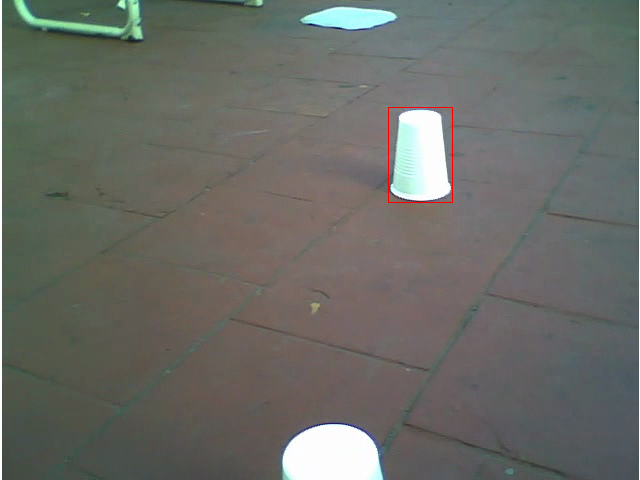
\includegraphics[scale=0.4]{vision/figures/ventana-1.png}
\end{center}
  \caption[Ventaneo]{\small Se observa un vaso delimitado por un rect\'angulo 
  contenedor m\'inimo rojo. El rect\'angulo se utiliza para calcular el 
  tama\~no de la sub-imagen previo al ventaneo.}
  \label{fig:ventaneo}
\end{figure}


\begin{figure}[htpb]
\begin{center}
  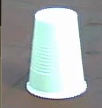
\includegraphics[scale=0.6]{vision/figures/ventana-2.png}
\end{center}
  \caption[Ejemplo de ventana]{\small Ventana o sub-imagen obtenida de un vaso en 
  focalizaci\'on. El tama\~no de la ventana es de tama\~no proporcional al 
  contorno del objeto en cuesti\'on.}
  \label{fig:ventaneo_2}
\end{figure}

	
	
\subsection{Resultados}
En esta secci\'on se describen los par\'ametros utilizados para la 
medici\'on de la performance y se muestran los resultados obtenidos para 
el sistema de visi\'on y un sistema de visi\'on con predicci\'on. De este 
\'ultimo exhibimos dos configuraciones. Tomamos 8 videos de prueba en los cuales 3 pertenecen a 
colillas, 3 a vasos y 2 a platos. Los videos fueron tomados utilizando 
una silla de oficina giratoria para poder desplazarse suavemente por 
el entorno simulando el movimiento del robot. La c\'amara se ubic\'o a 30 
cm del piso formando un \'angulo de $30^{\circ}$ con el asiento  en direcci\'on 
hacia el suelo. La c\'amara utilizada es una microsoft lifecam vx-700 del tipo webcam y posee una 
resoluci\'on de 640x480.

\subsubsection{Par\'ametros de medici\'on}
Con el objetivo de  medir la efectividad del algoritmo de detecci\'on, desarrollamos un sistema de benchmarking. Este sistema permite
a un usuario indicar la presencia de objetos a detectar en un video, marc\'andolos con rect\'angulos en las sucesiones de cuadros. De esta
manera, corremos el algoritmo de detecci\'on por el mismo video y verificamos que los centroides de los objetos detectados por el algoritmo 
se encuentren contenidos dentro de los rect\'angulos indicados por el 
usuario. Para obtener estad\'isticas sobre la performance  
medimos los siguientes par\'ametros:
\begin{itemize}
\item { Cantidad de objetos a detectar \textbf{(\#O)}: Se corresponde con la cantidad de rect\'angulos marcados por el usuario}
\item { Hits\textbf{(H)} : Cantidad de detecciones por parte del algoritmo que se corresponden con rect\'angulos marcados.}
\item { Misses o detecciones falsas \textbf{(M)} : Cantidad de detecciones por parte del algoritmo que no se corresponden con rect\'angulos marcados.}
\end{itemize}
Se desprende directamente, de estos valores, que la cantidad de detecciones: 
\textbf{$\#D=H+M$} .
Con estos datos obtenemos los porcentajes de error, falsos positivos : 
\[
	fp=1 - \frac{H}{\# O}
\]
y falsos negativos:
\[
	fn=\frac{M}{\# D}
\]
En el caso \'optimo, ambas medidas de error tendr\'an un valor de $0\%$.  \\
\indent A estas estad\'isticas se agregan las particulares para el sistema de predicci\'on. Recolectamos informaci\'on sobre
cu\'antos casos el sistema de predicci\'on estim\'o la posici\'on y acert\'o . Denominamos
a la cantidad de estimaciones realizada por el sistema de predicci\'on 
con \textbf{G} mientras que a las estimaciones que adem\'as fueron 
acertadas \textbf{G\&H}.

\subsubsection{An\'alisis}
Exhibimos los resultados obtenidos tras utilizar s\'olo el sistema de 
visi\'on en el cuadro \ref{tab:result} e utilizando el sistema de 
visi\'on con el sistema de predicci\'on, utilizando dos configuraciones 
distintas, en 
los cuadros \ref{tab:pred} y  \ref{tab:pred_2}. Adem\'as exhibimos los 
resultados promedios de falsos positivos y falsos negativos agrupados 
por objeto para todas las configuraciones en los cuadros \ref{tab:evo_colillas}, 
\ref{tab:evo_vasos} y \ref{tab:evo_platos}. Las configuraciones 
utilizadas fueron seleccionadas para destacar distintos comportamientos del 
sistema de predicci\'on. Éstas son:
\begin{itemize}
\item{\textbf{Configuraci\'on 1:} $\lambda=10$, $\rho=10$, $\delta=3$}
	\item{\textbf{Configuraci\'on 2:} $\lambda=10$, $\rho=4$, $\delta=2$}
\end{itemize}
\indent En los resultados arrojados en el cuadro \ref{tab:result} 
(s\'olo por el sistema de visi\'on) observamos problemas en la  detecci\'on de colillas ya que posee altos 
porcentajes de falsos negativos. Esto indica que el detector, en el 
caso de las colillas, tiene
problemas en distinguir a estas de su entorno ya que comete 
demasiados errores al reconocer colillas que no existen. Esto concuerda 
con el hecho de que, en el caso de las colillas, el n\'umero de 
detecciones \#D es siempre mayor que \#O tambi\'en observado en el 
cuadro \ref{tab:result}. No obstante, al utilizar el sistema de 
predicci\'on observamos una gran reducci\'on de este porcentaje producto 
del filtrado realizado por dicho sistema el cual no considera una 
basura hasta que esta est\'e presente en $\delta$ cuadros consecutivos.  
Esta mejora viene acompa\~nada de efecto negativos ya que la cantidad de 
hits se ve afectada pero con menor intensidad. Esto prueba que el 
filtrado realizado es efectivo ya que elimina, sobre el total de las 
detecciones, en mayor proporci\'on a 
aquellas que son falsas. El cuadro \ref{tab:evo_colillas} exhibe las ventajas de utilizar un sistema de 
predicci\'on para las colillas.\\
\indent 
En el caso de los vasos, observamos que el sistema de visi\'on brinda 
una muy buena performance por s\'i solo, como se ve en el cuadro \ref{tab:result} 
donde se muestran valores menores al $10\%$ en falsos positivos y falsos 
negativos para todos los videos. La diferencia de performance con la 
detecci\'on de colillas es comprensible ya que los vasos poseen 
caracter\'isticas como tama\~no y color que hacen que sea m\'as f\'acil 
reconocerlos y mas dif\'icil confundirlos en relaci\'on con estas 
\'ultimas, que poseen un color similar al del fondo y son de tama\~no 
peque\~no. En este caso, el sistema de predicci\'on no altera demasiado 
los resultados como en el caso de las colillas, sin embargo, destacamos un 
aumento en la cantidad de detecciones falsas en la configuraci\'on 1, 
atribuido a el valor elevado de $\rho$, acompa\~nado de un incremento 
similar en el porcentaje de aciertos. Distinto es el caso de 
la configuraci\'on 2 que disminuye levemente el porcentaje de falsas 
detecciones y el porcentaje de aciertos respecto de los resultados
obtenidos por el sistema de visi\'on. El comportamiento de la 
configuraci\'on 2 es razonable ya que esta es menos 
invasiva\footnote{Nos referimos a una configuraci\'on menos invasiva en 
el sentido de que la presencia del sistema de predicci\'on no modifica 
dr\'asticamente los resultados arrojados por el sistema de visi\'on.} y m\'as respetuosa del sistema de visi\'on subyacente en 
comparaci\'on con la configuraci\'on 1. Esto se ve reflejado, en parte, 
en la cantidad de estimaciones ( \textbf{G} ) y estimaciones correctas 
(\textbf{G\&H}) cometidas por cada configuraci\'on. Podemos 
apreciar las diferencias entre las distintas configuraciones para los 
vasos en el cuadro \ref{tab:evo_vasos}.\\
\indent El caso de los platos es similar al de los vasos. El sistema de visi\'on 
obtiene buenos resultados por s\'i s\'olo pero se ve perjudicado por la configuraci\'on 1 del sistema de 
predicci\'on ya que \'este no acierta en gran proporci\'on de las estimaciones que realiza. 
Sin embargo, en este caso, el aumento en el porcentaje de detecciones 
falsas es relativamente mayor que el aumento de aciertos. 
La configuraci\'on 2, por otro lado, aumenta el 
porcentaje de aciertos y disminuye la cantidad de detecciones falsas 
aunque en ambos casos, de manera leve, mejorando apenas los resultados 
obtenidos por el sistema de visi\'on. En este caso, los porcentajes de 
aciertos de las estimaciones son bajos pero observamos que utilizando 
la configuraci\'on 2 el n\'umero de estimaciones es mucho menor con lo 
que se cometen menos errores. Un cuadro comparativo de las 
distintas configuraciones para vasos pueden observarse en el cuadro 
\ref{tab:evo_platos}.\\
\indent  Las dos configuraciones del sistema de predicci\'on modifican de 
distintas maneras al algoritmo de visi\'on subyacente. Para cada objeto 
hemos obtenido resultados y comportamiento particulares lo que 
justifica la necesidad de ajustar los par\'ametros del mismo para obtener la mejor 
performance posible. Para poder realizar este ajuste es necesario 
establecer que grado de incidencia tienen los dos tipos de errores en la performance del
algoritmo. Por ejemplo, bajo distintas circunstancias podemos preferir que el  
sistema de visi\'on cometa m\'as errores de tipo I (falsos positivos) con 
el objetivo de minimizar errores de tipo II ( falsos negativos) o 
viceversa. En ese sentido el sistema de predicci\'on proporciona los mecanismos que 
permiten lograr estos ajustes sin necesidad de modificar el algoritmo de detecci\'on 
subyacente. Para nuestro caso, por lo explicado en \ref{comp_conclusion}, priorizamos 
la disminuci\'on en los errores de tipo I frente a los de tipo II y ,por lo tanto, configurar\'iamos
el sistema de predicci\'on acorde.\\
\indent En cuanto al tiempo de procesamiento demandado por el algoritmo obtuvimos
una velocidad de procesamiento de aproximadamente $8.3$ $cuadros/seg$ s\'olo utilizando
el sistema de visi\'on en conjunto con el sistema de predicci\'on. No obstante, como hemos explicado
en \ref{sec:focaliz}, los mecanismos de focalizaci\'on y ventaneo reducen notablemente la
complejidad del algoritmo una vez que se enfoca un residuo.
 

%~ Esto se lo atribuimos a que esta configuraci\'on tiene un valor de 
%~ $\rho$ elevado y por lo tanto modifica demasiado la performance del 
%~ sistema de visi\'on. Recordemos que a valores de $\rho$ m\'as elevados, 
%~ mayor ser\'an el n\'umero de estimaciones de la posici\'on de los objetos 
%~ siendo m\'as propenso a cometer errores. En el caso de los vasos, debido 
%~ a la alta efectividad del sistema de visi\'on, resulta contra-producente  
%~ arriesgar tanto. Esto se verifica utilizando la configuraci\'on 2 donde 
%~ ,al realizar una menor cantidad de estimaciones, se obtiene un n\'umero mucho 
%~ menor de detecciones falsas sin comprometer tanto la cantidad de 
%~ aciertos. 
%~ caso de los vasos y platos que presentan porcentajes relativamente 
%~ bajos en todos los casos. La diferencia de performance entre los vasos 
%~ y platos con las colillas es esperable ya que las colillas son 
%~ objetos de menor tama\~no e incluso poseen un color muy similar al del 
%~ entorno, lo cual dificulta su detecci\'on. En cambio, el color blanco y 
%~ el gran tama\~no de los vasos y platos hace que se distingan f\'acilmente 
%~ del fondo pero su color los hace m\'as sensibles a la iluminaci\'on.\\
%~ \indent Utilizando el mismo sistema de visi\'on con el sistema de 
%~ predicci\'on  obtenemos resultados un tanto distintos indicados en la 
%~ tabla \ref{tab:pred}. En el caso de las colillas observamos una mejora notable 
%~ en los falsos negativos debido al efecto pasa-altos establecido por 
%~ la variable $\delta$, eliminando las apariciones espontaneas y el 
%~ n\'umero de detecciones en general. A su vez, esta disminuci\'on impacta 
%~ en la cantidad de hits y por consecuente en el porcentaje de falsos 
%~ negativos, pero de forma mucho m\'as leve lo que lo hace un trade-off 
%~ favorable. En el caso de los vasos y platos no se observa ninguna 
%~ mejora notoria. En los vasos vemos un leve incremento 
%~ en el porcentaje de falsos positivos producido por $\delta$ pero en 
%~ este caso, a diferencia de las colillas, la disminuci\'on en el 
%~ porcentaje de falsos negativos es a\'un m\'as peque\~na, resultando en un 
%~ balance no favorable. Algo similar sucede con los platos en donde se 
%~ reduce notablemente la cantidad de hits sin ver ninguna mejora en la 
%~ cantidad de detecciones falsas. Esto \'ultimo puede ser atribuido a la 
%~ gran cantidad de errores cometidos al estimar la posici\'on del objeto 
%~ cuando este no fue detectado por el sistema de visi\'on. En s\'intesis, el 
%~ sistema de predicci\'on logr\'o una influencia positiva en el detector de colillas
%~ filtrando algunas detecciones falsas pero entorpeci\'o la detecci\'on de vasos y platos
%~ donde ya pose\'iamos una buena performance. La configuraci\'on utilizada para el sistema de 
%~ predicci\'on en este cuadro result\'o muy invasiva para estos dos detectores y los forz\'o a 
%~ estimar posiciones de los objetos cuando esto no era necesario ya que se pose\'ia un n\'umero bajo de 
%~ deteccions falsas.\\
%~ \indent En el cuadro \ref{tab:pred_2} exhibimos los resultados obtenidos con un sistema de predicci\'on
%~ menos invasivo. En este caso se eligieron valores de $\lambda=10$, $\rho=4$ y $\delta=2$. Tomando un valor
%~ de $\rho$ y $\delta$ le damos m\'as confianza al sistema de visi\'on como fue explicado previamente. En los vasos y
%~ platos es notable la reducci\'on en la cantidad de falsas detecciones sin afectar demasiado el n\'umero de hits logrado.
%~ Esto viene acompa\~nado con el hecho de que el predictor realizo menos estimaciones y aumento su tasa de acierto en todos 
%~ los casos. Los resultados obtenidos para estos dos objetos son mejores que los obtenidos solo con el sistema de visi\'on. 
%~ Sin embargo, en el caso de las colillas, el predictor si impacto en la cantidad de hits por lo que no se observa un 
%~ cambio del todo favorable respecto de la configuraci\'on anterior.\\
\begin{table}[htb]
  \begin{tabular}{|l | c | c | c | c | c | c |}
	\hline  
	\textbf{Video} & \textbf{(\#O)} &  \textbf{(\#D)} & \textbf{(H)} & 
	\textbf{(M)} & \textbf{fp} & \textbf{fn}\\
	\hline
	\hline
	vasos1 & 5050 & 4880 & 4849 & 31 & 0.6\% & 3.9\% \\
	vasos2 & 1777 & 1708 & 1696 & 12 & 0.7\% & 4.5\% \\	
	vasos3 & 6196 & 5354 & 5251 & 103 & 1.9\% & 15.2\% \\
	\hline
	colillas1 & 1645 & 1648 & 1282 & 367 & 22.2\% & 22.0\% \\
	colillas2 & 891 & 1045 & 636 &  409 & 39.1\% & 28.6\% \\
	colillas3 & 2708 & 3899 & 2373 & 1526 & 39.2\% & 12.7\% \\
	\hline
	platos1 & 2236 & 1966 & 1832 & 134 & 6.8\% & 18.0\%\\
	platos2 & 1128 & 1228 & 1117 & 111& 9.0\% & 0.9\% \\
	\hline
	\end{tabular}
	\caption[Performance del algoritmo de visi\'on]{\label{tab:result} Performance del sistema sin el algoritmo de predicci\'on}
\end{table}

%Con predicci\'on
\begin{table}[htb]
  \begin{tabular}{|l | c | c | c | c | c | c | c | c |}
	\hline  
	\textbf{Video} & \textbf{(\#O)} &  \textbf{(\#D)} & \textbf{(H)} & \textbf{(M)} & \textbf{fp} & \textbf{fn} & \textbf{G} & \textbf{G\&H} \\
	\hline
	\hline
	vasos1 & 5050 & 5017 & 4888 & 118 & 2.3\% & 3.2\%  & 245 & 142\\
	vasos2 & 1777 & 1773 & 1707 & 66 & 3.7\% & 3.9\% & 121 & 60 \\
	vasos3 & 6196 & 5703 & 5459 & 240 & 4.2\% & 11.8\% & 536 & 373 \\
	\hline
	colillas1 & 1645 & 1444 & 1330 & 98 & 6.8\% & 19.1\% & 296 & 229 \\
	colillas2 & 891 & 687 & 586 & 95 & 13.9\% & 34.2\% & 127 & 57 \\
	colillas3 & 2708 & 2555 & 2242 & 254 & 10.1\% & 17.2  & 516 & 320\\
	\hline
	platos1 & 2236 & 1966 & 1854 & 218 & 10.5\% & 17.0\% & 179 & 34\\
	platos2 & 1128 & 1228 & 1112 & 167& 13.0\% & 1.4\% & 115 & 16\\
	\hline
	\end{tabular}
	\caption[Performance con sistema de predicci\'on configuraci\'on 1]{\label{tab:pred} Performance del sistema con el sistema de predicci\'on para 
	$\lambda=10$, $\rho=10$, $\delta=3$ }
\end{table}

\begin{table}[htb]
  \begin{tabular}{|l | c | c | c | c | c | c | c | c |}
	\hline  
	\textbf{Video} & \textbf{(\#O)} &  \textbf{(\#D)} & \textbf{(H)} & \textbf{(M)} & \textbf{fp} & \textbf{fn} & \textbf{G} & \textbf{G\&H} \\
	\hline
	\hline
	vasos1 & 5050 & 4866 & 4839 & 27 & 0.5\% & 4.1\%  & 83 & 72\\
	vasos2 & 1777 & 1700 & 1689 & 11 & 0.6\% & 4.9\% & 32 & 27 \\
	vasos3 & 6196 & 5318 & 5222 & 96 & 1.8\% & 15.7\% & 241 & 226 \\
	\hline
	colillas1 & 1645 & 1220 & 1168 & 53 & 4.3\% & 28.9\% & 142 & 126 \\
	colillas2 & 891 & 652 & 566 & 86 & 13.1\% & 36.4\% & 78 & 38 \\
	colillas3 & 2708 & 2414 & 2142 & 272 & 11.2\% & 20.0\% & 303 & 158 \\
	\hline
	platos1 & 2236 & 1958 & 1843 & 115 & 5.8\% & 17.5\% & 50 & 16 \\
	platos2 & 1128 & 1211 & 1115 & 96 & 7.9\% & 1.1\% & 26 & 8 \\
	\hline
	\end{tabular}
	\caption[Performance con sistema de predicci\'on configuraci\'on 2]{\label{tab:pred_2} Performance del sistema con el sistema de predicci\'on con
	$\lambda=10$, $\rho=4$, $\delta=2$}
\end{table}

\begin{table}[h]
  \begin{tabular}{|l | c | c | c | c | c|}
	\hline  
	\textbf{Configuraci\'on} & \textbf{$\bar{fp}$} &  
	\textbf{$\bar{fn}$}& \textbf{G} &  \textbf{G\&H} &  \textbf{G\&H/G} \\
	\hline
	\hline
	Sin predicci\'on  & 18.1\% & 34.9\% & - & - & - \\
	\hline
	Configuraci\'on 1 & 20.7\% & 9.5\% & 939 & 606 & 64.5\%  \\
	\hline
	Configuraci\'on 2 & 26.0\% & 9.5\% & 523 & 322 & 61.5\% \\
	\hline
	\end{tabular}
	\caption[Performance promedio de las colillas]{\label{tab:evo_colillas} Performance promedio de las colillas 
	por configuraci\'on y  efectividad de las estimaciones del sistema de predicci\'on}
\end{table}

\begin{table}[h]
  \begin{tabular}{|l | c | c | c | c | c|}
	\hline
	\textbf{Configuraci\'on} & \textbf{$\bar{fp}$} &  \textbf{$\bar{fn}$}& \textbf{G} &  \textbf{G\&H} &  \textbf{G\&H/G} \\
	\hline
	\hline
	Sin predicci\'on  & 9.4\% & 1.2\% & - & - & -\\
	\hline
	Configuraci\'on 1 & 7.4\% &	3.3\% & 902 & 575 & 63.7\% \\
	\hline
	Configuraci\'on 2 & 9.7\% &	1.1\% & 356 & 325 & 91.2\%\\
	\hline
	\end{tabular}
	\caption[Performance promedio de los vasos]{\label{tab:evo_vasos} Performance promedio de los vasos seg\'un configuraci\'on del 
	sistema y efectividad de las estimaciones del sistema de predicci\'on}
\end{table}



\begin{table}[h]
  \begin{tabular}{|l | c | c | c | c | c|}
	\hline
	\textbf{Configuraci\'on} & \textbf{$\bar{fp}$} &  \textbf{$\bar{fn}$}& \textbf{G} &  \textbf{G\&H} &  \textbf{G\&H/G} \\
	\hline
	\hline
	Sin predicci\'on &  12.3\% & 7.6\% & - & - & -\\
	\hline
	Configuraci\'on 1 & 11.8\% & 12.0\% & 294 & 50 & 17.0\%\\
	\hline
	Configuraci\'on 2 & 12.0\% & 6.6\% & 76 & 24 & 31.5\% \\
	\hline
	\end{tabular}
	\caption[Performance promedio de los platos]{\label{tab:evo_platos} Performance promedio de los platos seg\'un configuraci\'on del 
	sistema y efectividad de las estimaciones del sistema de predicci\'on}
\end{table}



\subsection{Conclusi\'on}
Presentamos un algoritmo para el reconocimiento de distintos objetos en 
un ambiente din\'amico en el marco de un robot aut\'onomo capaz de 
recolectar basura. El mismo funciona sobre la librer\'ia de visi\'on 
computacional OpenCV y el lenguaje C++.  El algoritmo cuenta
con una etapa de pre-procesado donde se extraen los pixeles de colores de inter\'es y se disminuye el ruido utilizando 
operaciones morfol\'ogicas y de threshold. La etapa de procesamiento extrae los contornos y utiliza una aproximaci\'on por pol\'igonos
para simplificar el an\'alisis posterior. Este consiste en una serie de 
filtros pre-definidos dispuestos en cascada que interpretan la 
informaci\'on de contorno y  determinan si se trata 
de un objeto de inter\'es o no. 
Implementamos un mecanismo de predicci\'on parametrizable que funciona 
sobre el algoritmo en cuesti\'on por el cual se puede optimizar la performance de 
detecci\'on seg\'un las caracter\'isticas propias de cada detector. Se 
midieron los resultados obtenidos realizando el reconocimiento de 
vasos, colillas y platos obteniendo un promedio de $14\%$ de falsos 
positivos  y $5\%$ de falsos negativos. Finalmente agregamos un mecanismo de focalizaci\'on por el cual 
el sistema completo puede concentrarse sobre un \'unico objeto reduciendo 
los tiempos de procesamiento. 


\subsubsection{Posibles extensiones}
Existen varios puntos donde consideramos se pude mejorar este sistema 
de reconocimiento de objetos. Una de las \'areas donde se pueden introducir mejoras es en 
la secci\'on de filtros. Como hemos visto, existen novedosas t\'ecnicas de 
descripci\'on y representaci\'on de contornos que pueden ser introducidas 
como un filtro adicional sin necesidad de modificar la estructura del 
algoritmo. La utilizaci\'on de dichas t\'ecnicas pueden servir para 
la caracterizaci\'on de nuevos objetos a reconocer o bien para reforzar 
los objetos ya tratados. Por otro lado, hallamos al sistema de filtros 
en cascada un tanto limitado para la tarea propuesta ya que frente a 
peque\~nas perturbaciones que provoquen que un \'unico filtro rechaze un 
determinado contorno, este \'ultimo se ver\'a descartado por el sistema. 
Como alternativas a este sistema se puede implementar un sistema de 
votaci\'on donde se re\'unan los resultados de cada filtro y se tome una 
decisi\'on en base a ellos. Adicionalmente, ser\'ia interesante que en 
este sistema de votaci\'on se pueda indicar un valor que establezca la 
importancia de cada filtro en relaci\'on a un objeto determinado. Otra 
posibilidad, bas\'andonos en el trabajo \cite{potato} expuesto en la 
secci\'on \ref{volunteer}, es utilizar las 
caracter\'isticas medidas por los filtros para entrenar un clasificador. 
Luego este ser\'a capaz de caracterizar a los residuos utilizando los 
valores medidos de manera \'optima.\\
\indent En lo que respecta a la etapa de pre-procesamiento se pueden 
tomar las ideas del trabajo \cite{sidewalk2008} expuesto en la secci\'on \ref{sec:sidewalk} 
para caracterizar el entorno del robot. Esto es, mantener histogramas 
que modelen el entorno del robot utilizando aquellas regiones de las 
im\'agenes donde no se hallaron  objetos de inter\'es. De este modo ser\'ia m\'as f\'acil 
distinguir un objeto del fondo o entorno que lo rodea. Esto tambi\'en 
ayudar\'ia al algoritmo de visi\'on a adaptarse a los cambios de 
iluminaci\'on que pueden ocurrir ya que este histograma se podr\'ia 
actualizar peri\'odicamente.\\
\indent Introducir alg\'un sistema de sensado por el cual el robot pueda 
detectar si efectivamente se ha recolectado un residuo reconocido o no, resulta de 
gran inter\'es ya que permitir\'ia implementar alg\'un mecanismo de 
aprendizaje por refuerzo para el sistema de visi\'on. De esta manera, el 
sistema de visi\'on podr\'ia adaptar par\'ametros como el valor del umbral en las
operaciones de filtrado, el rango en el canal de tono para el filtro de color o los l\'imites 
superiores e inferiores en el filtro de \'area de acuerdo a los 
refuerzos recibidos.\\
\indent El sistema de predicci\'on puede cometer errores cuando, por 
efectos de iluminaci\'on o oclusi\'on, un objeto cambia su \'area o 
per\'imetro en gran proporci\'on. Por lo tanto, la inclusi\'on de otros 
\emph{descriptores de contorno} en este sistema podr\'ia resultar en un 
seguimiento m\'as efectivo de los mismos a lo largo de los cuadros. 
Tambi\'en es posible mejorar la estimaci\'on de las posiciones utilizando 
f\'ormulas que tengan en cuenta no solo el \'ultimo desplazamiento sino 
el desplazamiento promedio del objeto en los \'ultimos cuadros.


